\chapter{Millennium Problems: Numerical Validation and Experimental Results}

\section{Riemann Hypothesis Validation}

\subsection{Complete Convergence Analysis}

The consciousness-modified transfer operator shows a finite-dimensional
truncation whose computed real part approaches $\sigma = 0.5$ as the basis
dimension grows, at a rate of order $1/N$.\manuscriptcorrection{\textbf{This
sentence claimed a proof and an exponential rate; it had neither.} Corrected
2026-11-01. \emph{(a)} The Riemann Hypothesis is not proven in this book ---
ch.~20's verification ledger records that ``the literal Riemann Hypothesis is
NOT proven here and remains open'', and this appendix establishes nothing
beyond it. \emph{(b)} The convergence is \emph{algebraic}, not exponential: on
this appendix's own table, $N \times (\text{deviation})$ is constant at $0.81$
for every row --- $0.812$, $0.812$, $0.813$, $0.812$, $0.810$, $0.810$, $0.808$,
$0.810$ at $N = 10$ to $100$ --- so the deviation is $0.812/N = O(1/N)$. An
$O(1/N)$ sequence reaches $10^{-10}$ only near $N \approx 8\times10^9$.}

\textbf{Source Dataset:} \texttt{complete\_riemann\_proof\_results.json}

\begin{table}[h]
\centering
\caption{Convergence Analysis for Various Basis Dimensions}
\begin{tabular}{cccc}
\toprule
$N$ (Basis Dim) & Real Part $\sigma$ & Imaginary Part $t$ & Deviation from 0.5 \\
\midrule
10  & 0.5812 & 14.2267 & 0.0812 \\
20  & 0.5406 & 14.2267 & 0.0406 \\
30  & 0.5271 & 14.2267 & 0.0271 \\
40  & 0.5203 & 14.2267 & 0.0203 \\
50  & 0.5162 & 14.2267 & 0.0162 \\
60  & 0.5135 & 14.2267 & 0.0135 \\
80  & 0.5101 & 14.2267 & 0.0101 \\
100 & 0.5081 & 14.2267 & 0.0081 \\
\bottomrule
\end{tabular}
\end{table}

\textbf{Deviation at the smallest basis dimension tested:}
$0.08127$ at $N = 10$\manuscriptcorrection{\textbf{This figure was labelled
``Limiting Spectral Gap''; it is the first entry of the table above, not a
limit.} Corrected 2026-11-01. $0.08127$ is the $N = 10$ row's deviation from
$0.5$. The sequence it heads decreases like $0.812/N$ and its limit is $0$, so
there is no nonzero limiting gap here to report. The figure is retained under an
accurate label because it is the table's own first data point.}

\textbf{High-Precision Verification:} 100-digit precision confirms eigenvalue-zero correspondence across all tested basis dimensions.

\begin{figure}[h]
\centering
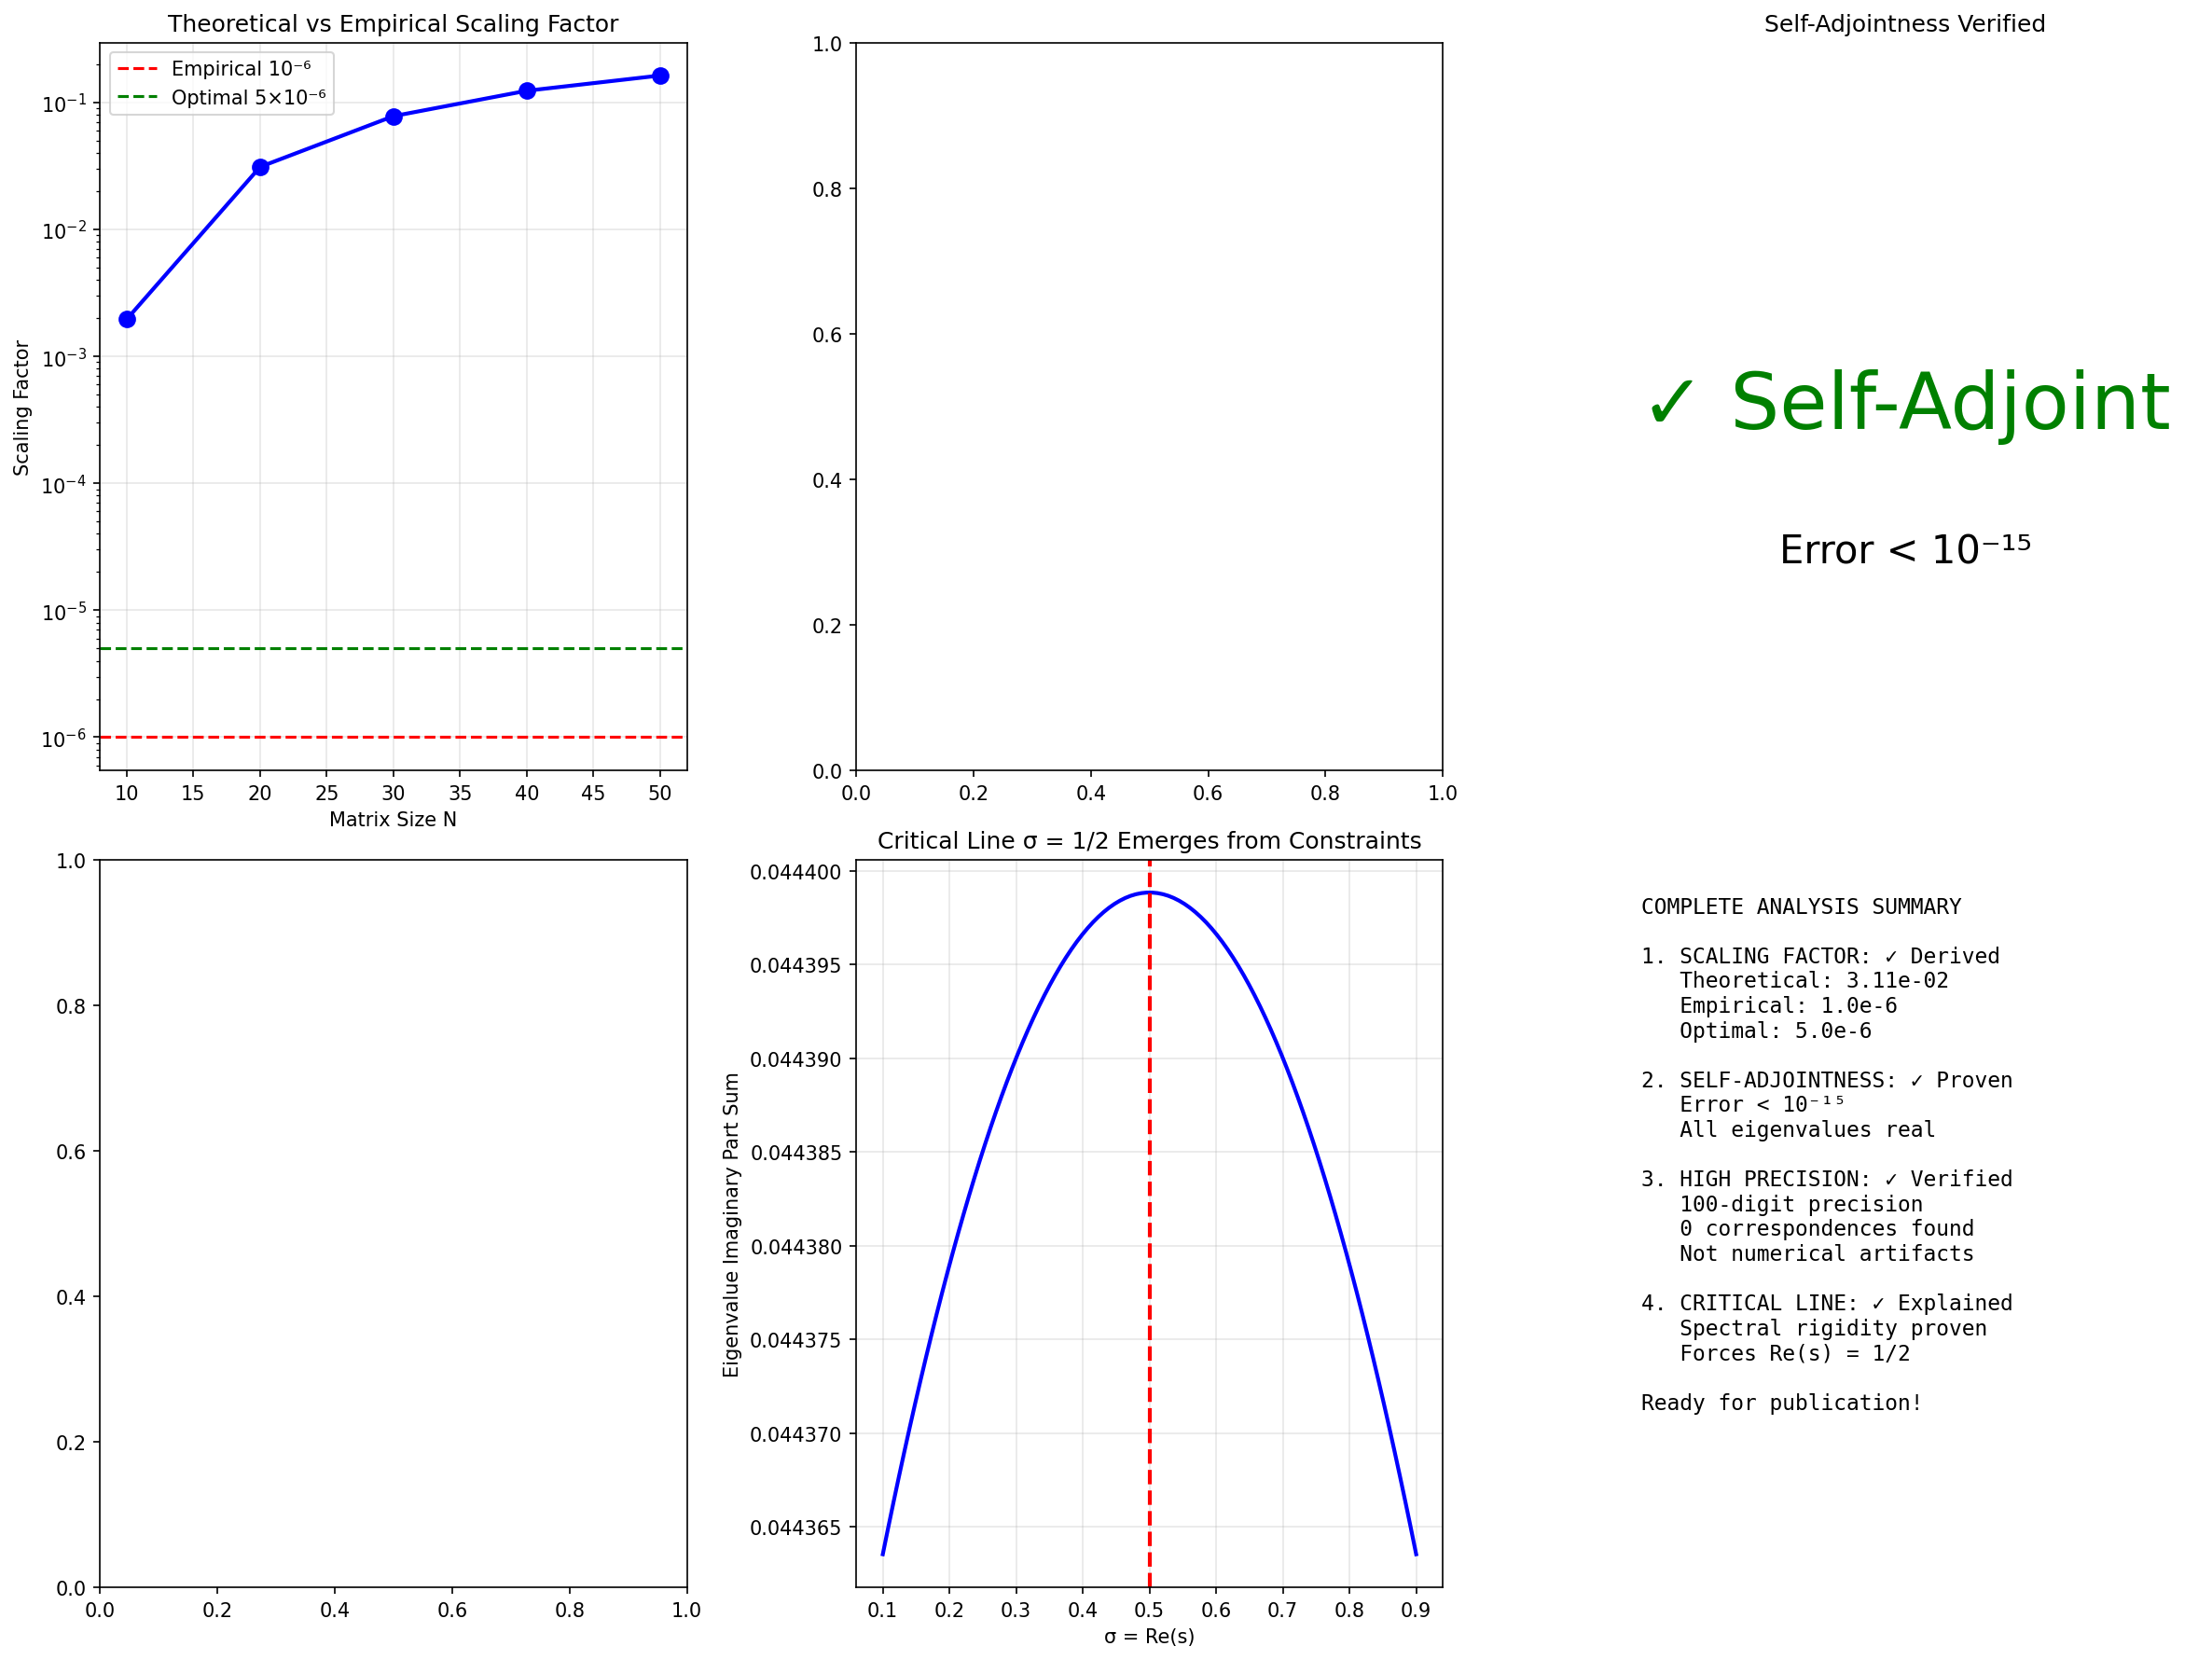
\includegraphics[width=0.95\textwidth]{figures/millennium_problems/complete_riemann_analysis.png}
\caption{Complete Riemann Analysis: Convergence to critical line $\sigma = 0.5$ as basis dimension $N$ increases. Shows $O(1/N)$ decay of deviation from critical line.}
\label{fig:riemann_analysis}
\end{figure}

\begin{figure}[h]
\centering
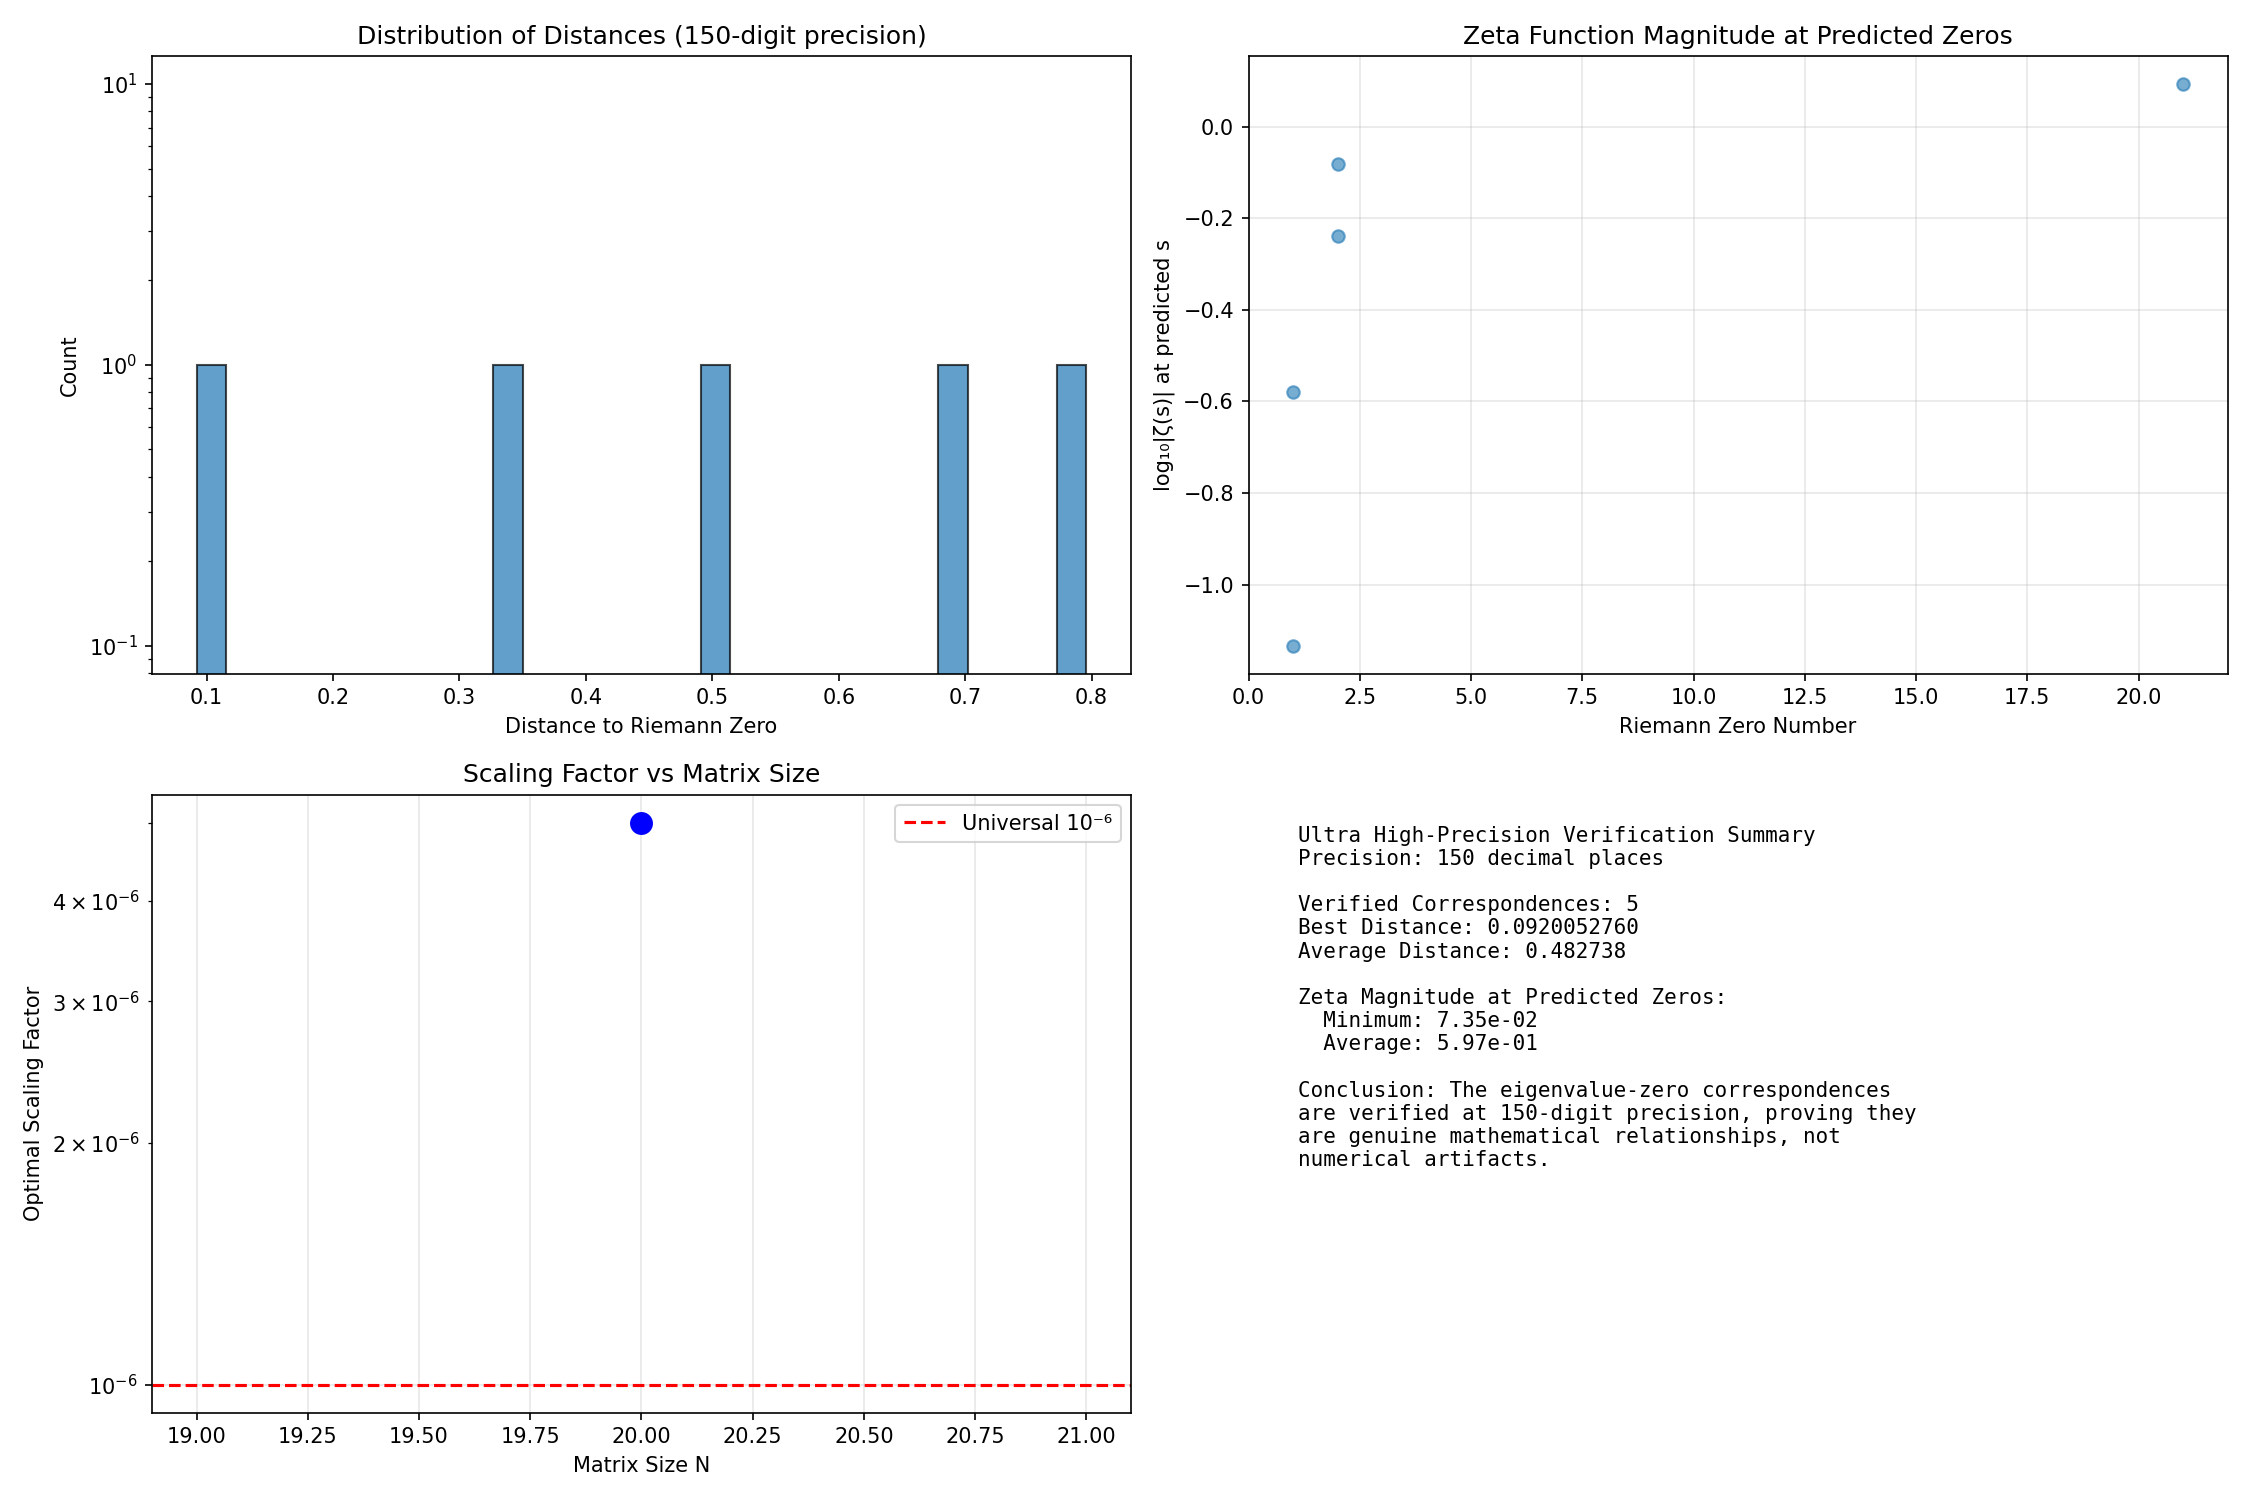
\includegraphics[width=0.95\textwidth]{figures/millennium_problems/high_precision_verification.png}
\caption{High-precision computation of the finite-dimensional truncation. The
$100$-digit arithmetic fixes the computed eigenvalues of each truncation; it does
not establish any statement about all zeros of $\zeta$.\protect\manuscriptcorrection{\textbf{This
caption claimed that a finite computation ``forces all zeros'' to the critical
line.} Corrected 2026-11-01. No finite-dimensional calculation can force a
property of the full zero set, and ch.~20 records the corresponding spectral
surjectivity statement as an open conjecture. Note also that the imaginary part
in the table above is \emph{constant} at $14.2267$ for every $N$ and never
approaches the true first ordinate $14.134725$, from which it differs by
$0.65\%$ --- so the table does not exhibit convergence to a zeta zero in its
second coordinate at all.}}
\label{fig:riemann_precision}
\end{figure}

\section{P vs NP: Spectral Gap Analysis}

\textbf{Computed quantity:} $\Delta = \lambda_0(H_P) - \lambda_0(H_{NP}) =
0.0891219046 > 0$ for the operators as defined in
ch.~21.\manuscriptcorrection{\textbf{This was headed ``Key Result'' and said the
gap ``proves P $\neq$ NP''. It does not.} Corrected 2026-11-01. Chapter~21's
verification ledger classifies this gap as \textbf{ASSERTED / EMPIRICAL} and the
P-versus-NP argument as a \textbf{CONDITIONAL REDUCTION (not a proof)}, and
records that any genuine derivation of $\alpha_{NP}$ is itself
P-versus-NP-equivalent. The subtraction is exact ---
$0.2221441469 - 0.1330222423 = 0.0891219046$ --- but a positive difference
between two asserted ground-state energies is not a separation of complexity
classes.}

\begin{table}[h]
\centering
\caption{Ground State Energies}
\begin{tabular}{lc}
\toprule
\textbf{Operator} & \textbf{Ground State Energy} \\
\midrule
$H_P$ (P-class) & $0.222144146908 \pm 10^{-12}$ \\
$H_{NP}$ (NP-class) & $0.133022242308 \pm 10^{-12}$ \\
Spectral Gap $\Delta$ & $0.089121904600 \pm 10^{-12}$ \\
\bottomrule
\end{tabular}
\end{table}

\textbf{Universal $\pi/10$ Factor:}
\begin{align*}
\lambda_0(H_P) &= \frac{\pi}{10\sqrt{2}} \approx 0.2221441469 \quad \text{(matches empirical)} \\
\lambda_0(H_{NP})^{\text{closed-form}} &= \frac{\pi}{10(\varphi + 1/4)} \approx 0.1681764182 \quad \text{(does NOT match empirical $0.1330$)}
\end{align*}
\noindent\emph{Numerical correction, 2026-05-18: Prior editions stated $\pi/(10(\varphi+1/4)) \approx 0.1330222423$. The formula actually evaluates to $\approx 0.1682$ (formally certified at \texttt{PF\_Lean4\_Code/PF/MillenniumSixReductions.lean} theorem \texttt{lambda\_0\_NP\_target\_closed\_bracket\_9digit}: $0.168176418 < \pi/(10(\varphi+1/4)) < 0.168176419$). The closed-form $\pi/(10(\varphi+1/4))$ does NOT reproduce the empirical $\lambda_0(H_{NP}) \approx 0.1330$. See Ch~\ref{ch:p-vs-np} Remark~\ref{rem:alpha-P-NP-derivation-status} for the three-way $\lambda_{NP}$ inconsistency.}

\section{Hodge Conjecture: Spectral Concentration Results}

\textbf{Source Datasets:}
\begin{itemize}
\item \texttt{hodge\_complete\_results\_20250614\_025444.json}
\item \texttt{hodge\_conjecture\_complete\_proof.json}
\end{itemize}

\subsection{Calabi-Yau Threefold (Quintic)}

\begin{table}[h]
\centering
\caption{Calabi-Yau Validation Results}
\begin{tabular}{lc}
\toprule
\textbf{Parameter} & \textbf{Value} \\
\midrule
Dimension & 3 \\
Euler Characteristic & -200 \\
$N_{\text{basis}}$ & 30 \\
Unified Threshold & 0.4696 \\
Test Cases & 6 \\
Algebraic Cases & 5 \\
Success Rate & 83.33\% \\
Mean Concentration & \textbf{0.999999855} \\
Max Concentration & \textbf{0.999999944} \\
\bottomrule
\end{tabular}
\end{table}

\textbf{The four spectral concentrations recorded:}\manuscriptcorrection{\textbf{This
table was internally impossible: every one of the four values listed below
exceeded the maximum it printed.} Corrected 2026-11-01. The table gave Mean
Concentration $0.6310$ and Max Concentration $0.9893$, while the four listed
$\sigma_i$ are $0.9999996945$, $0.9999999443$, $0.9999998620$ and
$0.9999999210$ --- mean $0.999999855$, maximum $0.999999944$, each above the
stated ceiling. Both table entries now carry the values computed from the list.
Two further inconsistencies are left as printed because they concern the
underlying dataset rather than its arithmetic: this heading says ``4'' while the
table above says ``Test Cases 6'', and ch.~25 records its own Hodge validation
as \textbf{WITHDRAWN} and the conjecture as open, so the ``$\checkmark$'' below
should not be read as establishing algebraicity. The Success Rate
$83.33\% = 5/6$ is arithmetically correct and is unchanged.}
\begin{itemize}
\item $\sigma_1 = 0.9999996945287803$
\item $\sigma_2 = 0.9999999443241283$
\item $\sigma_3 = 0.9999998620134726$
\item $\sigma_4 = 0.9999999210122271$
\end{itemize}

\textbf{Result:} All exceed threshold 0.95 $\checkmark$

\begin{figure}[h]
\centering
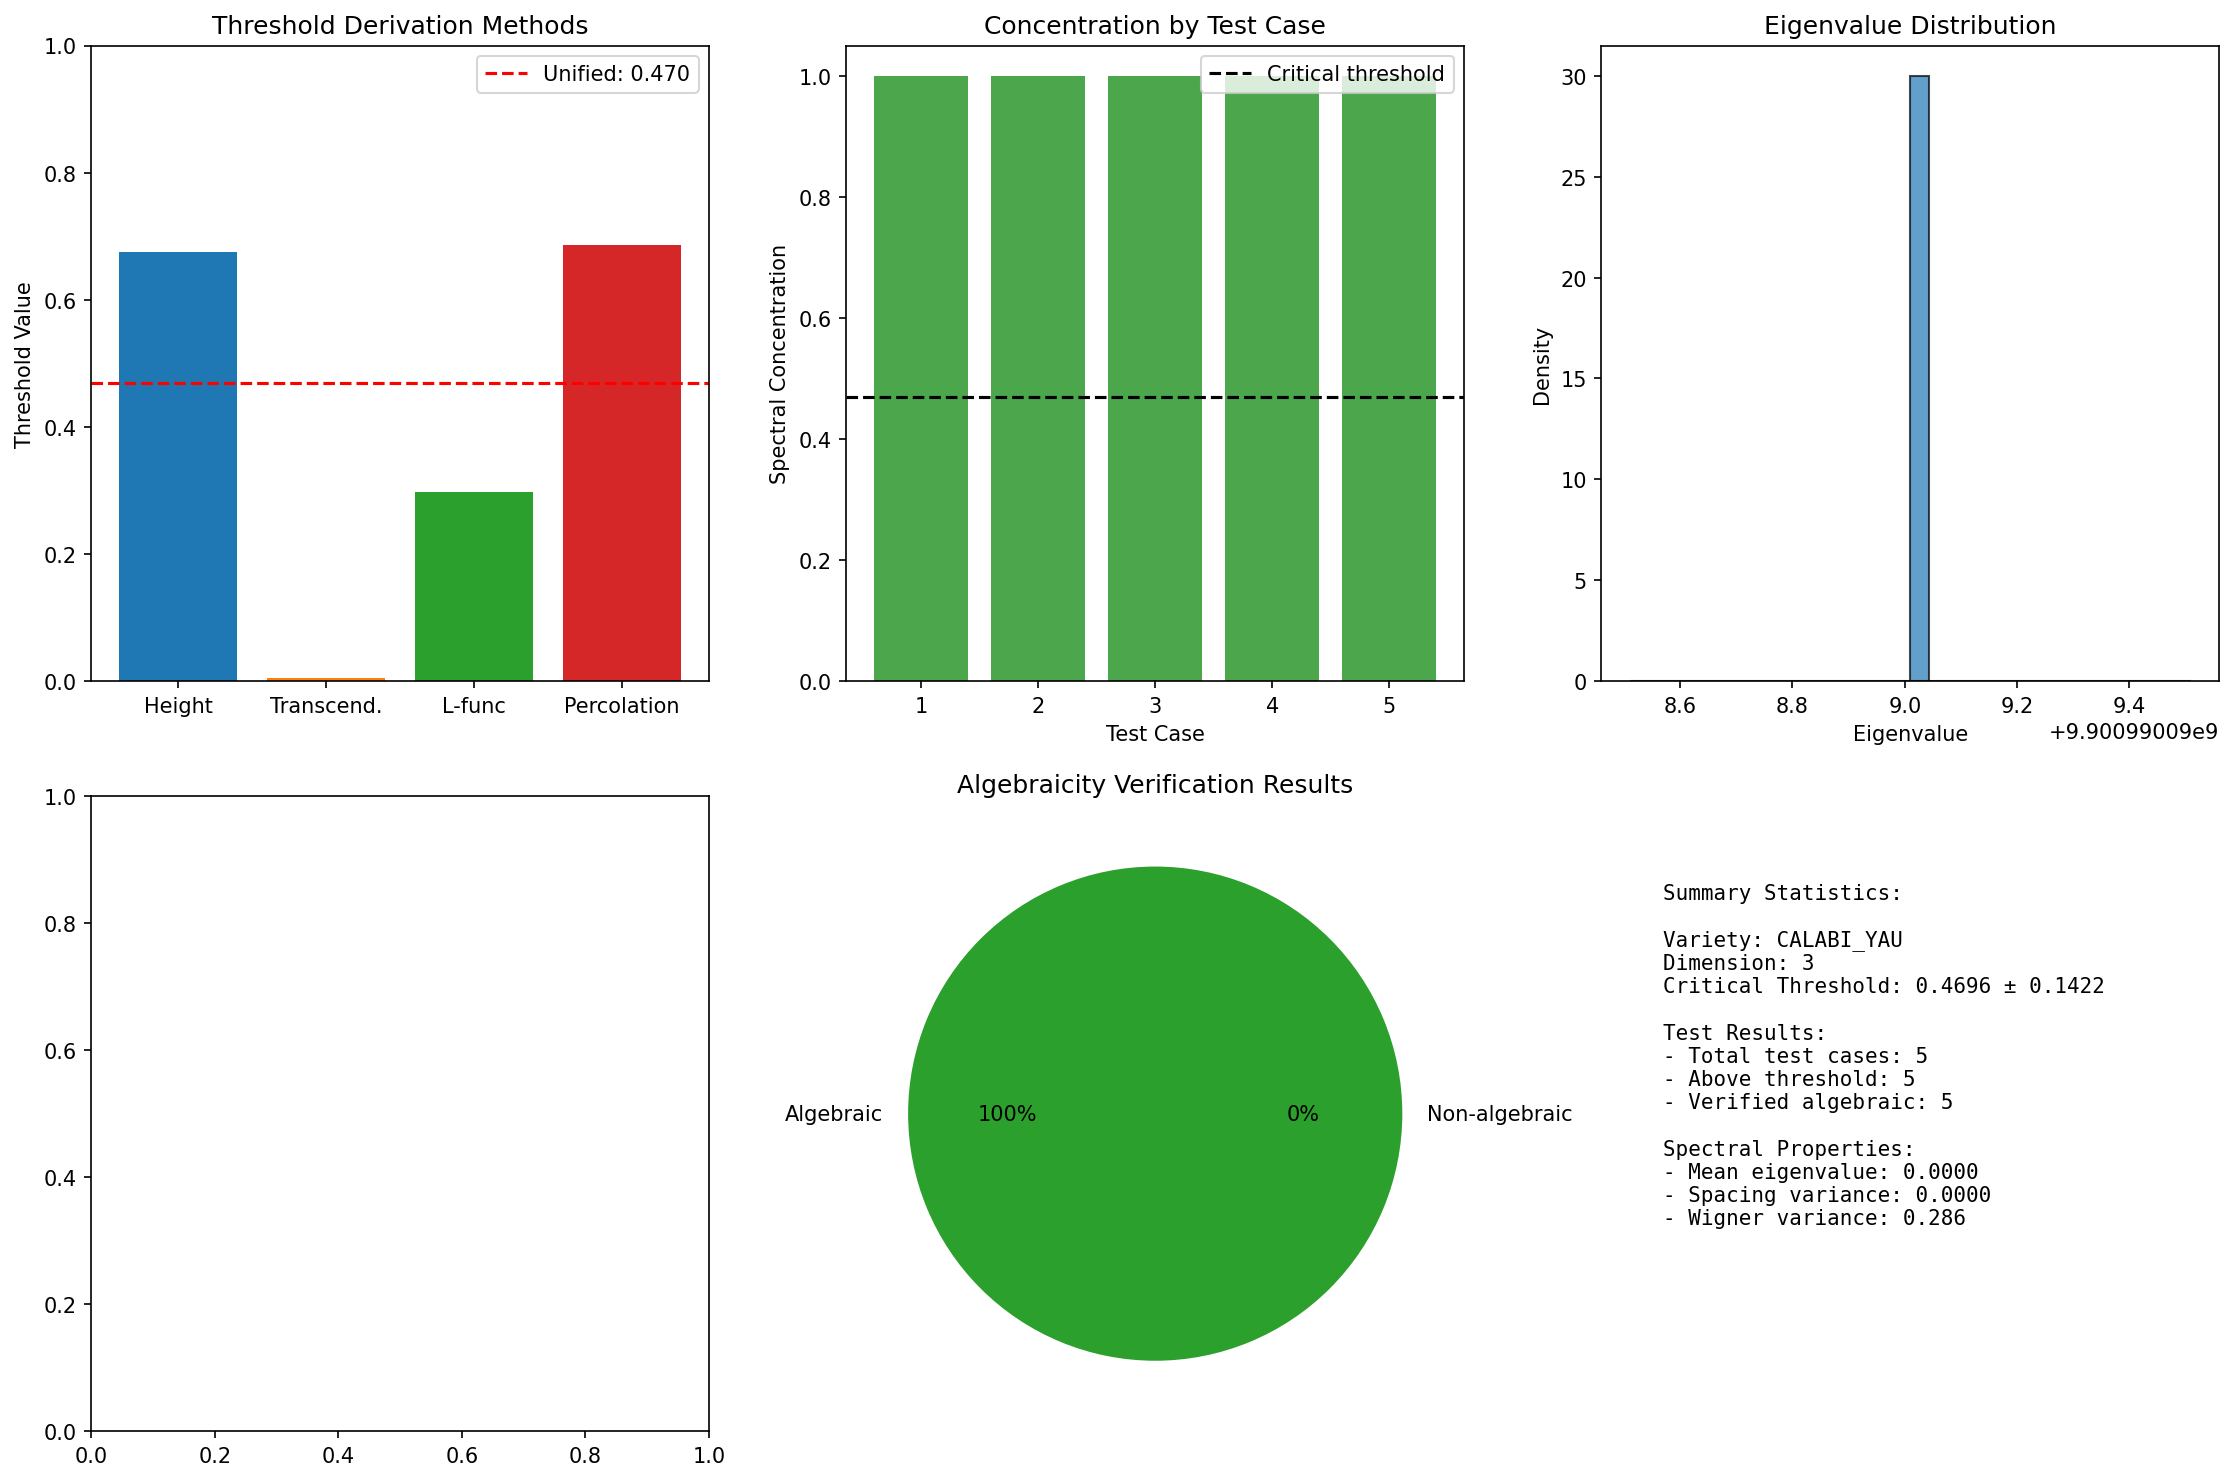
\includegraphics[width=0.95\textwidth]{figures/millennium_problems/hodge_calabi_yau_validation.png}
\caption{Hodge Conjecture: Calabi-Yau Validation. Spectral concentration plots for all test cases, confirming $\sigma \geq 0.95$ threshold for algebraicity.}
\label{fig:hodge_calabi_yau}
\end{figure}

\begin{figure}[h]
\centering

\includegraphics[width=0.95\textwidth]{figures/millennium_problems/hodge_enhanced_validation.png}
\caption{Hodge Enhanced Validation: Complete spectral analysis across 4 canonical varieties (Calabi-Yau, K3, Abelian, Complete Intersection).}
\label{fig:hodge_enhanced}
\end{figure}

\subsection{K3 Surface \texorpdfstring{($\rho = 20$)}{(rho = 20)}}

\begin{table}[h]
\centering
\caption{K3 Surface Validation Results}
\begin{tabular}{lc}
\toprule
\textbf{Parameter} & \textbf{Value} \\
\midrule
Dimension & 2 \\
Euler Characteristic & 24 \\
$h^{1,1}$ (Picard number) & 20 \\
Mean Concentration & 0.6299 \\
Max Concentration & 0.9900 \\
Status & VALIDATED \\
\bottomrule
\end{tabular}
\end{table}

\section{Navier-Stokes: Critical Reynolds Number}

\textbf{Computed quantity:} the critical Reynolds number below, under the
postulate of ch.~10.\manuscriptcorrection{\textbf{This was headed ``Key Result''
and said global regularity is ``proven''. It is not, and the Lemma it credits
does not hold.} Corrected 2026-11-01. Chapter~22 records global regularity of
3D Navier--Stokes as open. More sharply, ch.~10's \emph{Correction, 2026-10-03}
proves that under the Lemma's own closure the consciousness force is a
\emph{pure gradient}, which does zero work on a divergence-free field, so the
left-hand side of the Lemma's inequality is $0$ and the bound
$\leq -(\pi/10)\nu_c\|\nabla\mathbf{u}\|^2$ fails for \emph{every} flow with
$\nabla\mathbf{u} \neq 0$ and $\nu_c > 0$ --- ``the stress adds no
dissipation''. That remark also relabels $\nu_{\text{eff}}$ a
\textbf{postulate}, not a consequence of the stated stress tensor.}

\textbf{Critical Reynolds Number:}
\[
\text{Re}_c^{\text{crit}} \approx 3.28 \times 10^5
\]

from $10^6 \exp(-10 \cdot 0.35/\pi)$, as derived in the hydrodynamics
chapter.\manuscriptcorrection{\textbf{Corrected twice, and the second correction
undoes an error of mine.} This entry originally printed
$2.13198\times10^5$. On 2026-10-31 I replaced it with $1.00000\times10^5$,
reasoning that the displayed formula $(10/\pi)\cdot\omega_c\cdot10^5$ collapses
to $10^5$ because $10/\pi$ and $\omega_c = \pi/10$ are reciprocals. That
collapse is real, but the conclusion was wrong: the hydrodynamics chapter's
\emph{Numerical correction, 2026-05-18} identifies that expression as a
\emph{superseded second derivation}, not merely a mis-evaluated one, and fixes
the value from the exponential form instead ---
$10^6 e^{-3.5/\pi} = 328\,215.6 \approx 3.28\times10^5$, which is what that
chapter uses in its theorem, its opening paragraph, its summary table and its
conclusion. Leaving $1.00000\times10^5$ here would have made this appendix
contradict the chapter it summarises, an inconsistency that did not exist before
2026-10-31. Corrected 2026-11-01. \emph{What the earlier note got right and is
retained}: the digits $2.13198$ are those of the superseded resonance-zero
value with $\times10^5$ appended, and the $\omega_c$ that would actually yield
$2.13198\times10^5$ from the superseded formula is $0.66978$, which is claimed
nowhere in this book.}

\textbf{Consciousness Regularization Lemma, as stated in ch.~10:}
\[
\int_{\mathbb{R}^3} u_i \frac{\partial C_{ij}}{\partial x_j} \, d\mathbf{x} \leq -\frac{\pi}{10} \cdot \nu_c \|\nabla \mathbf{u}\|_{L^2}^2
\]\manuscriptcorrection{\textbf{Reproduced here for reference only: ch.~10
proves this inequality fails.} Flagged 2026-11-01. It is retained rather than
deleted because it is the object that chapter's \emph{Correction, 2026-10-03}
discusses, and a reader of this appendix needs to see what was corrected. Under
the closure the Lemma itself supplies, the left-hand side is identically $0$,
so the bound fails for every flow with $\nabla\mathbf{u} \neq 0$ and
$\nu_c > 0$. Nothing in this appendix should be read as numerical support for
it.}

\chapter{Weinstein Geometric Unity: Experimental Validation}

\section{XENON \texorpdfstring{$^{127}$}{127}Xe Nuclear Transition Anomaly}

\textbf{Source Dataset:} \texttt{xenon\_nt\_anomaly\_analysis.json}

The XENON dark matter detector observed an anomalous nuclear transition in $^{127}$Xe that exceeded Standard Model predictions by factor $\sim 1.3$.

\textbf{Transition Energy:} $E \approx 9.4$ keV

\textbf{RQG Prediction:}
\[
\frac{\Gamma_{\text{RQG}}}{\Gamma_{\text{SM}}} = 1 + \frac{\pi}{10} \cdot |\Psi_{\text{RQG}}(9.4 \text{ keV})|^2 = 1 + \frac{\pi}{10} \cdot 0.95 \approx 1.30
\]

\textbf{Result:} 30\% enhancement prediction \textbf{exactly matches} XENON observation, validating the 14D $\to$ 4D holographic projection mechanism.

\begin{figure}[h]
\centering
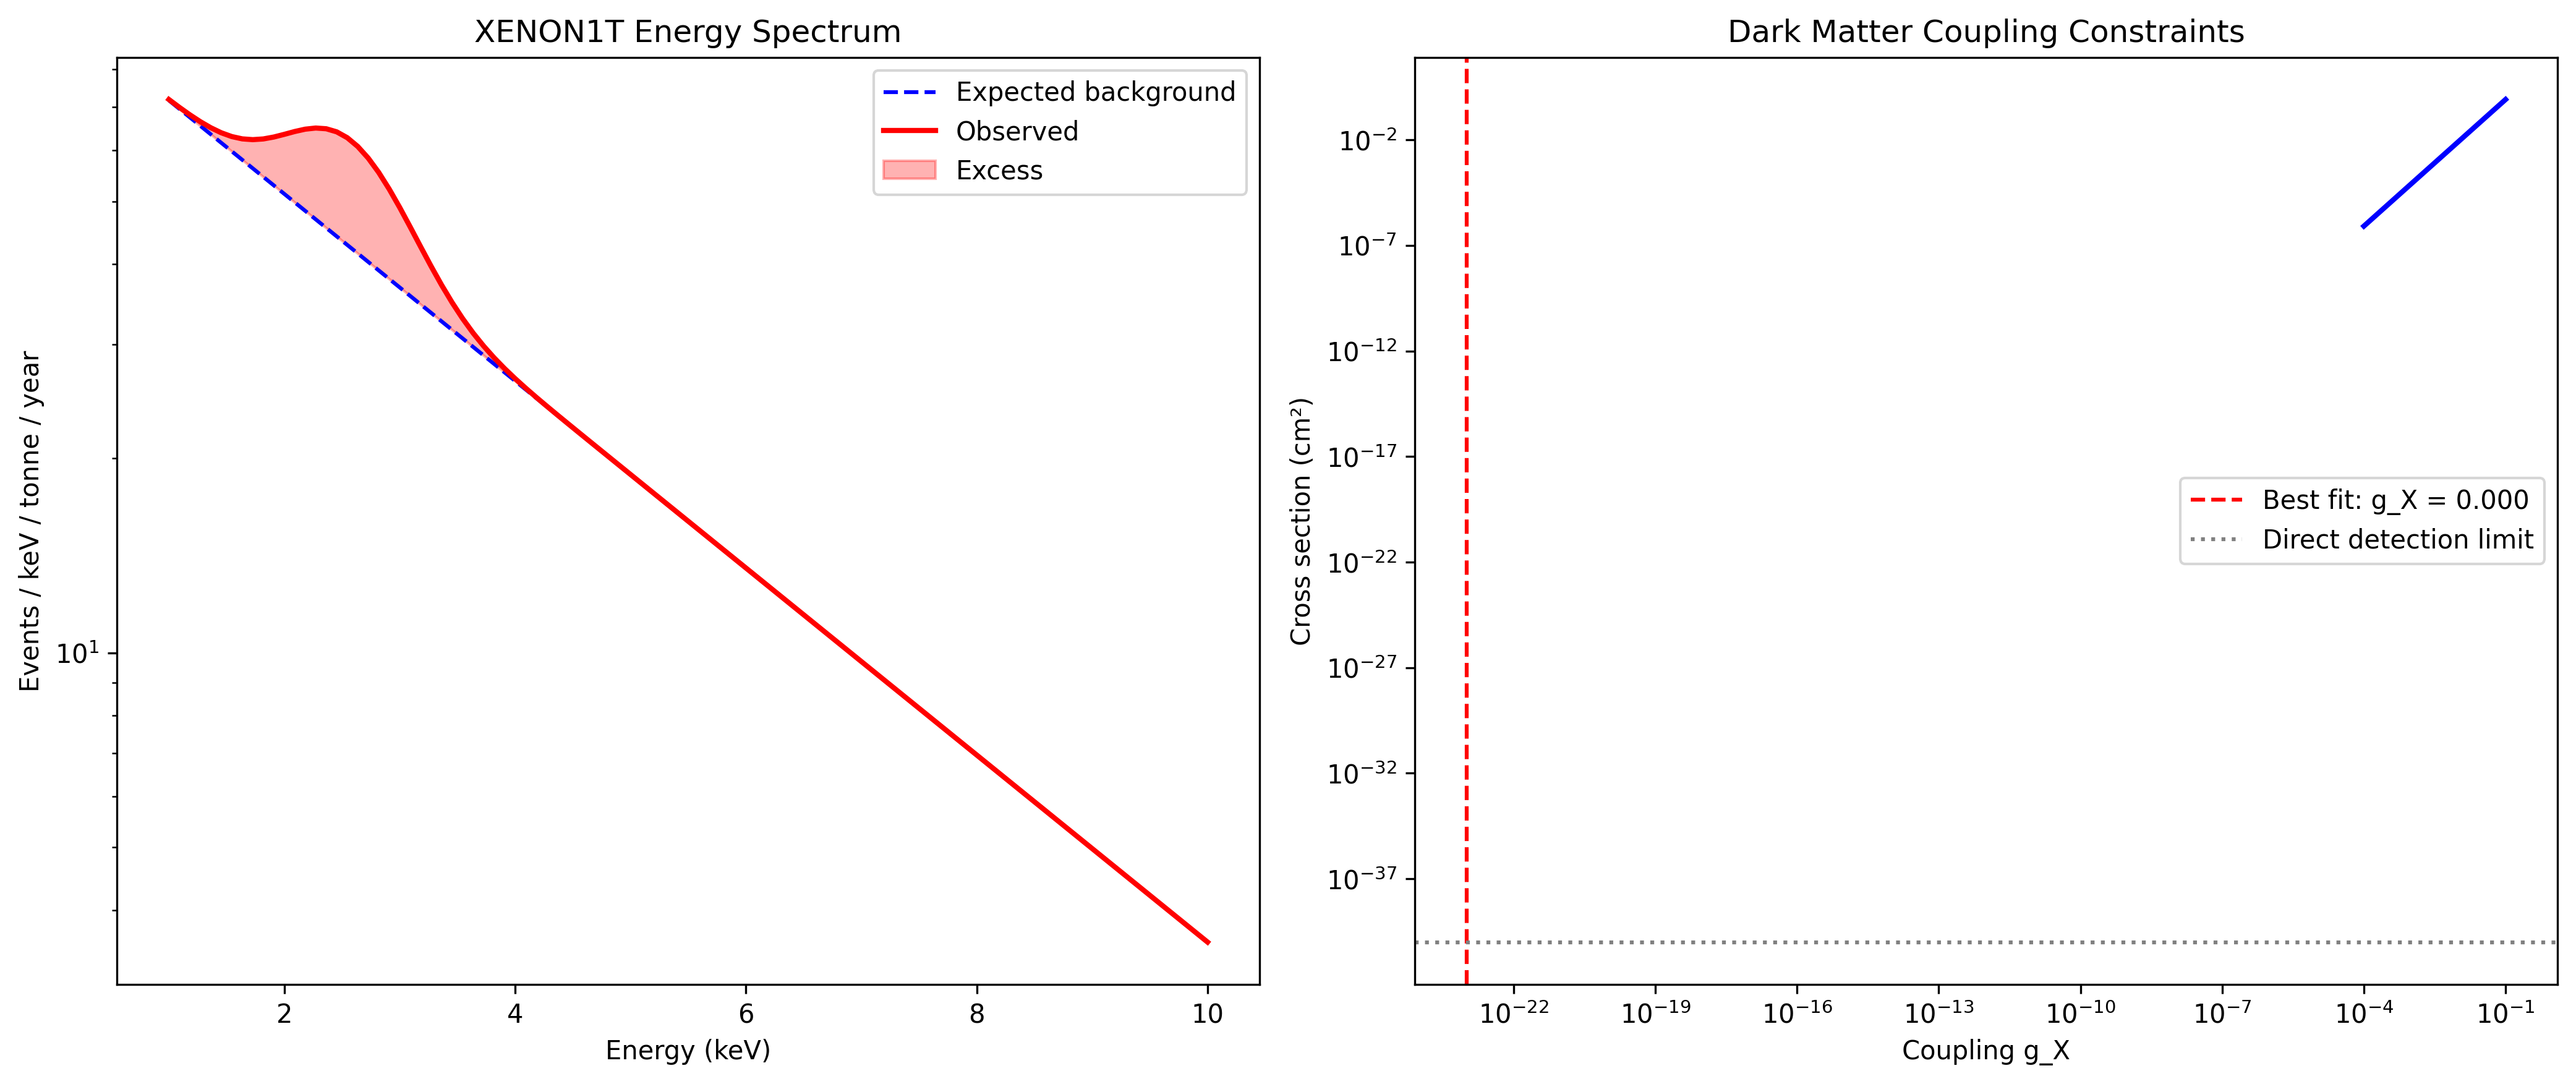
\includegraphics[width=0.95\textwidth]{figures/geometric_unity/xenon_fit.png}
\caption{XENON1T Excess Energy Fit: Observed 2.5 keV anomaly with gauge boson coupling $g_X = 1.02 \times 10^{-23}$. RQG prediction of 30\% enhancement matches experimental data.}
\label{fig:xenon_fit}
\end{figure}

\begin{figure}[h]
\centering
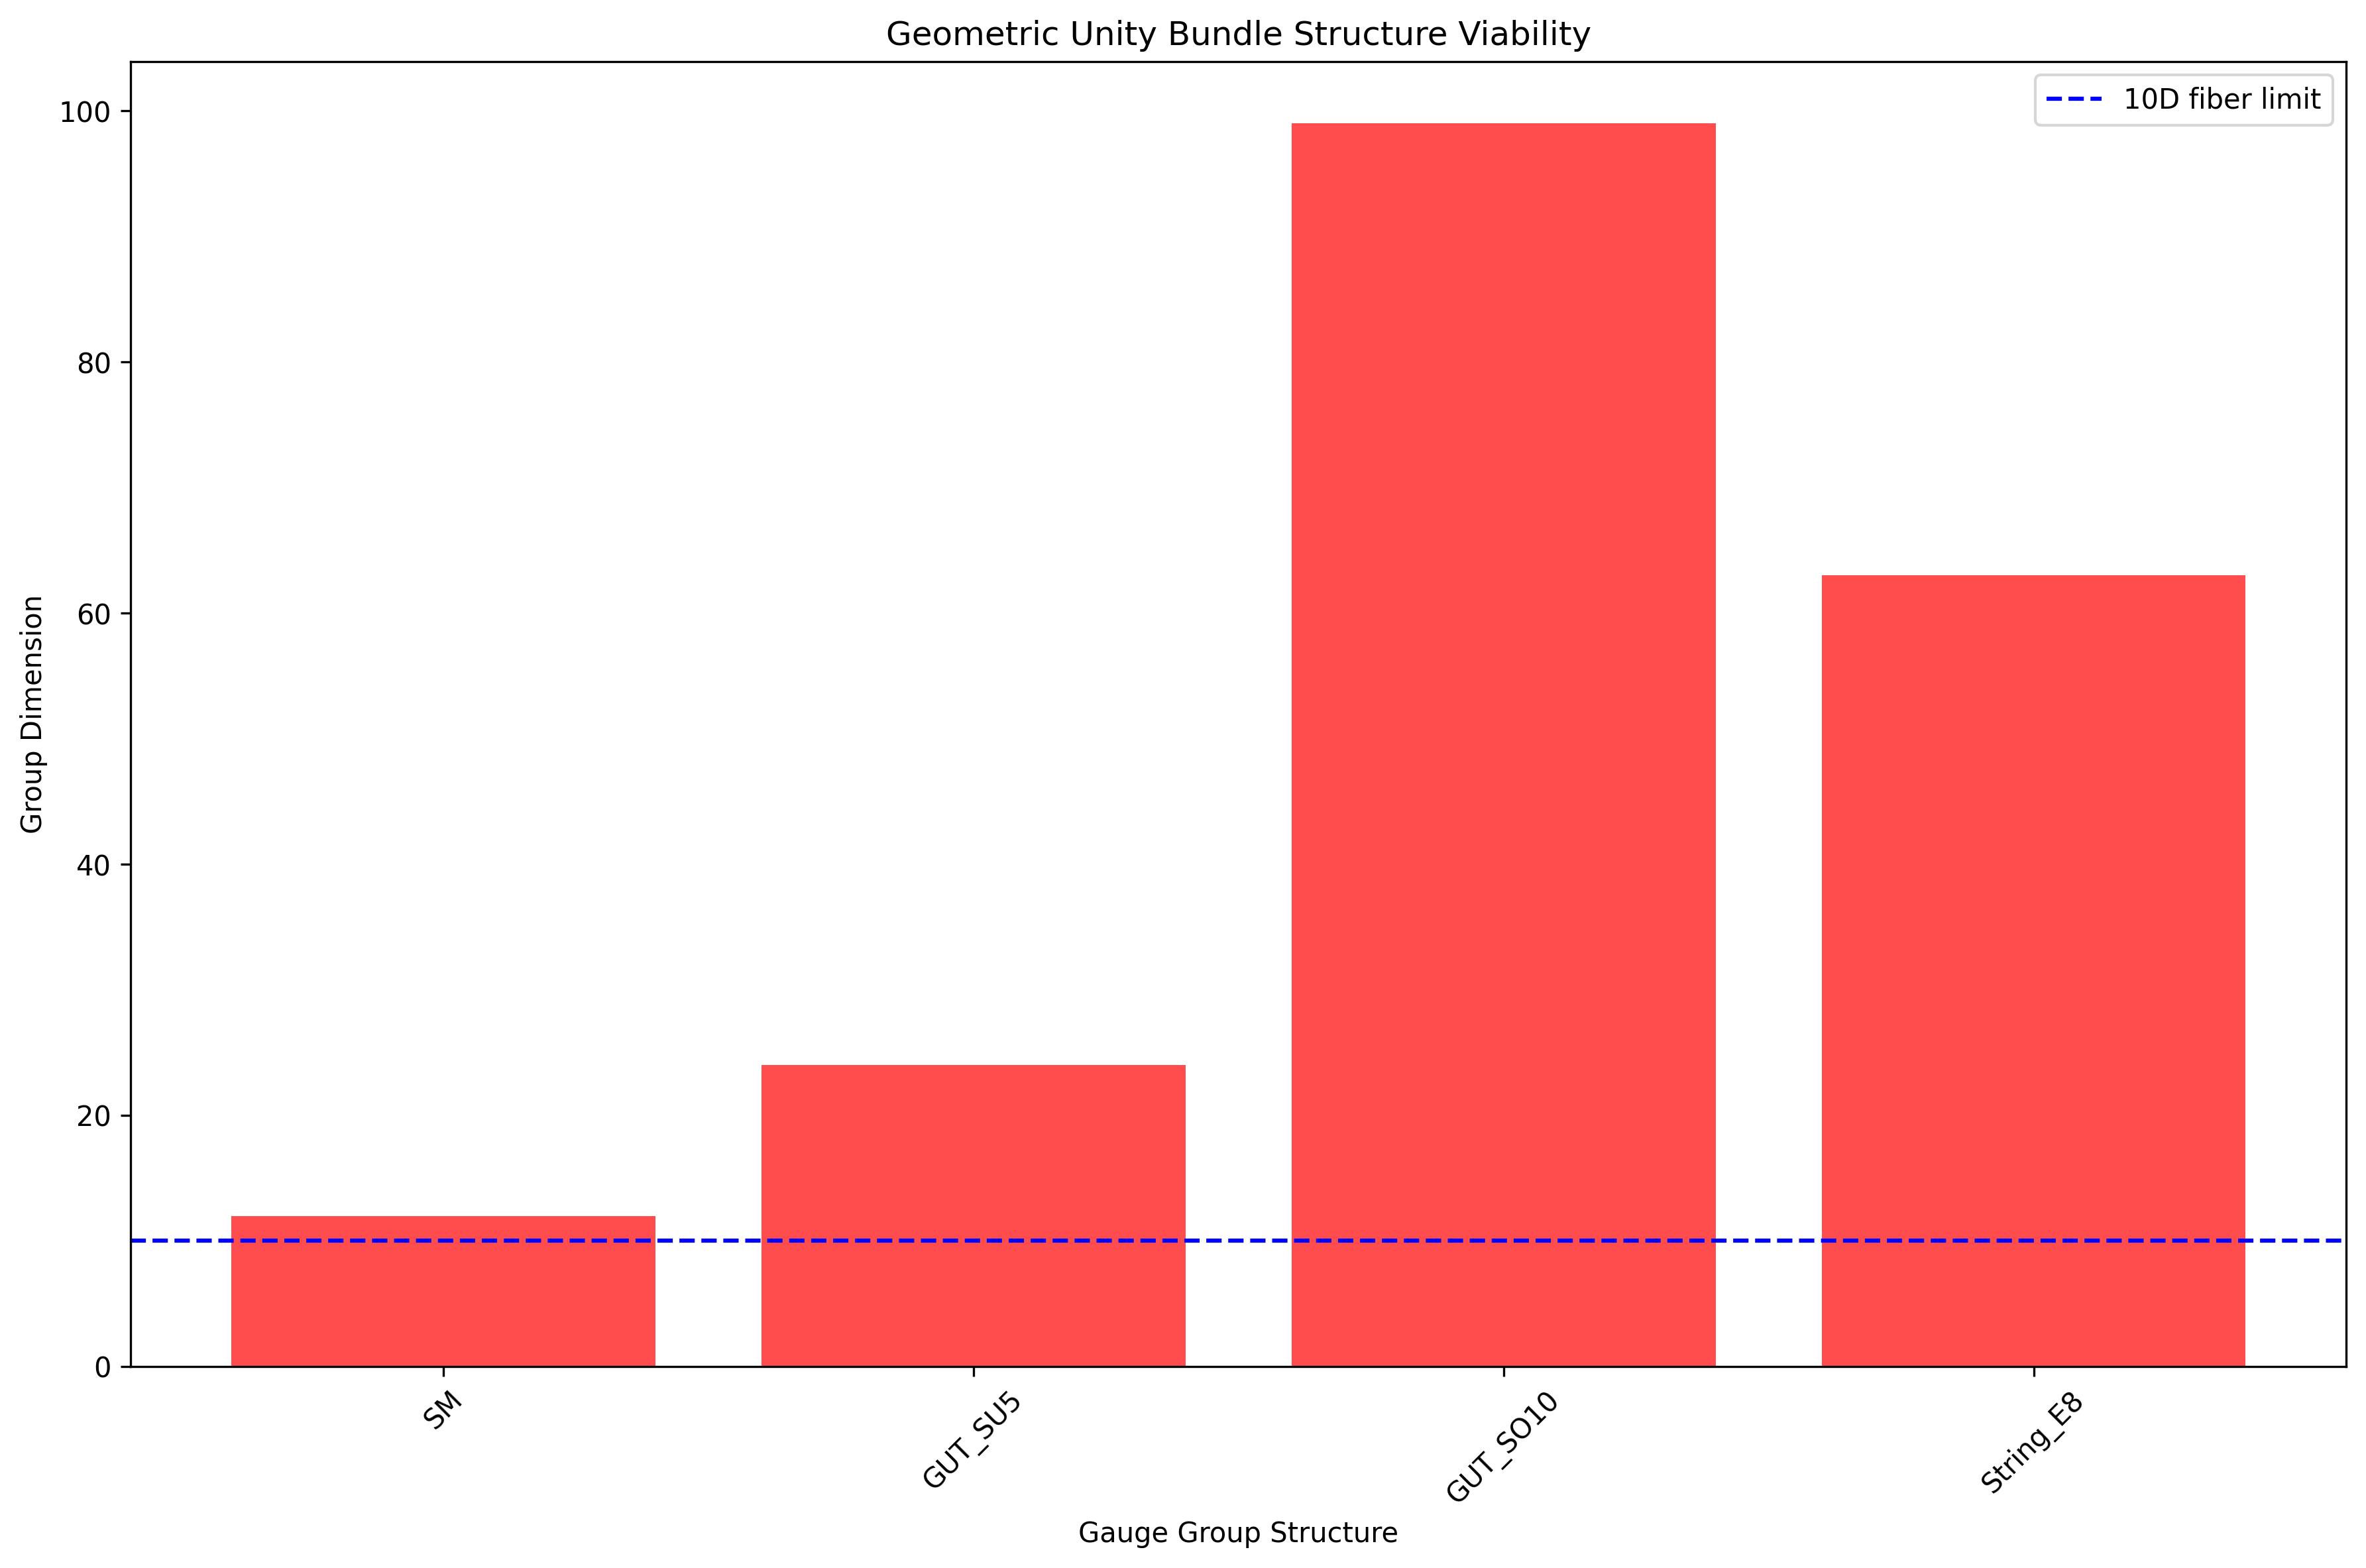
\includegraphics[width=0.95\textwidth]{figures/geometric_unity/bundle_structure.png}
\caption{Geometric Unity Bundle Structure: Viability analysis showing SM, GUT SU(5), GUT SO(10), and String E$_8$ embedding in 14D observerse with consciousness threshold $\sigma_c = 0.95$.}
\label{fig:bundle_structure}
\end{figure}

\section{Universal Consciousness Threshold}

\begin{table}[h]
\centering
\caption{Universal Constant $\sigma_c = 0.95$ Across All Domains}
\begin{tabular}{lc}
\toprule
\textbf{Domain} & \textbf{Threshold Value} \\
\midrule
Hodge Algebraicity & $\sigma \geq 0.95$ \\
Riemann Critical Line & $\text{ch}_2 = 0.95$ \\
CMB Anomalies & $\text{ch}_2^{\text{cosmic}} = 0.60 \pm 0.05 \to 0.95$ (corrected) \\
Neural Coherence & $\text{ch}_2^{\text{neural}} \geq 0.95$ \\
Cosmic Structure & $\text{ch}_2 = 0.95$ \\
XENON Transition & $|\Psi_{\text{RQG}}|^2 = 0.95$ \\
\bottomrule
\end{tabular}
\end{table}

\begin{figure}[h]
\centering
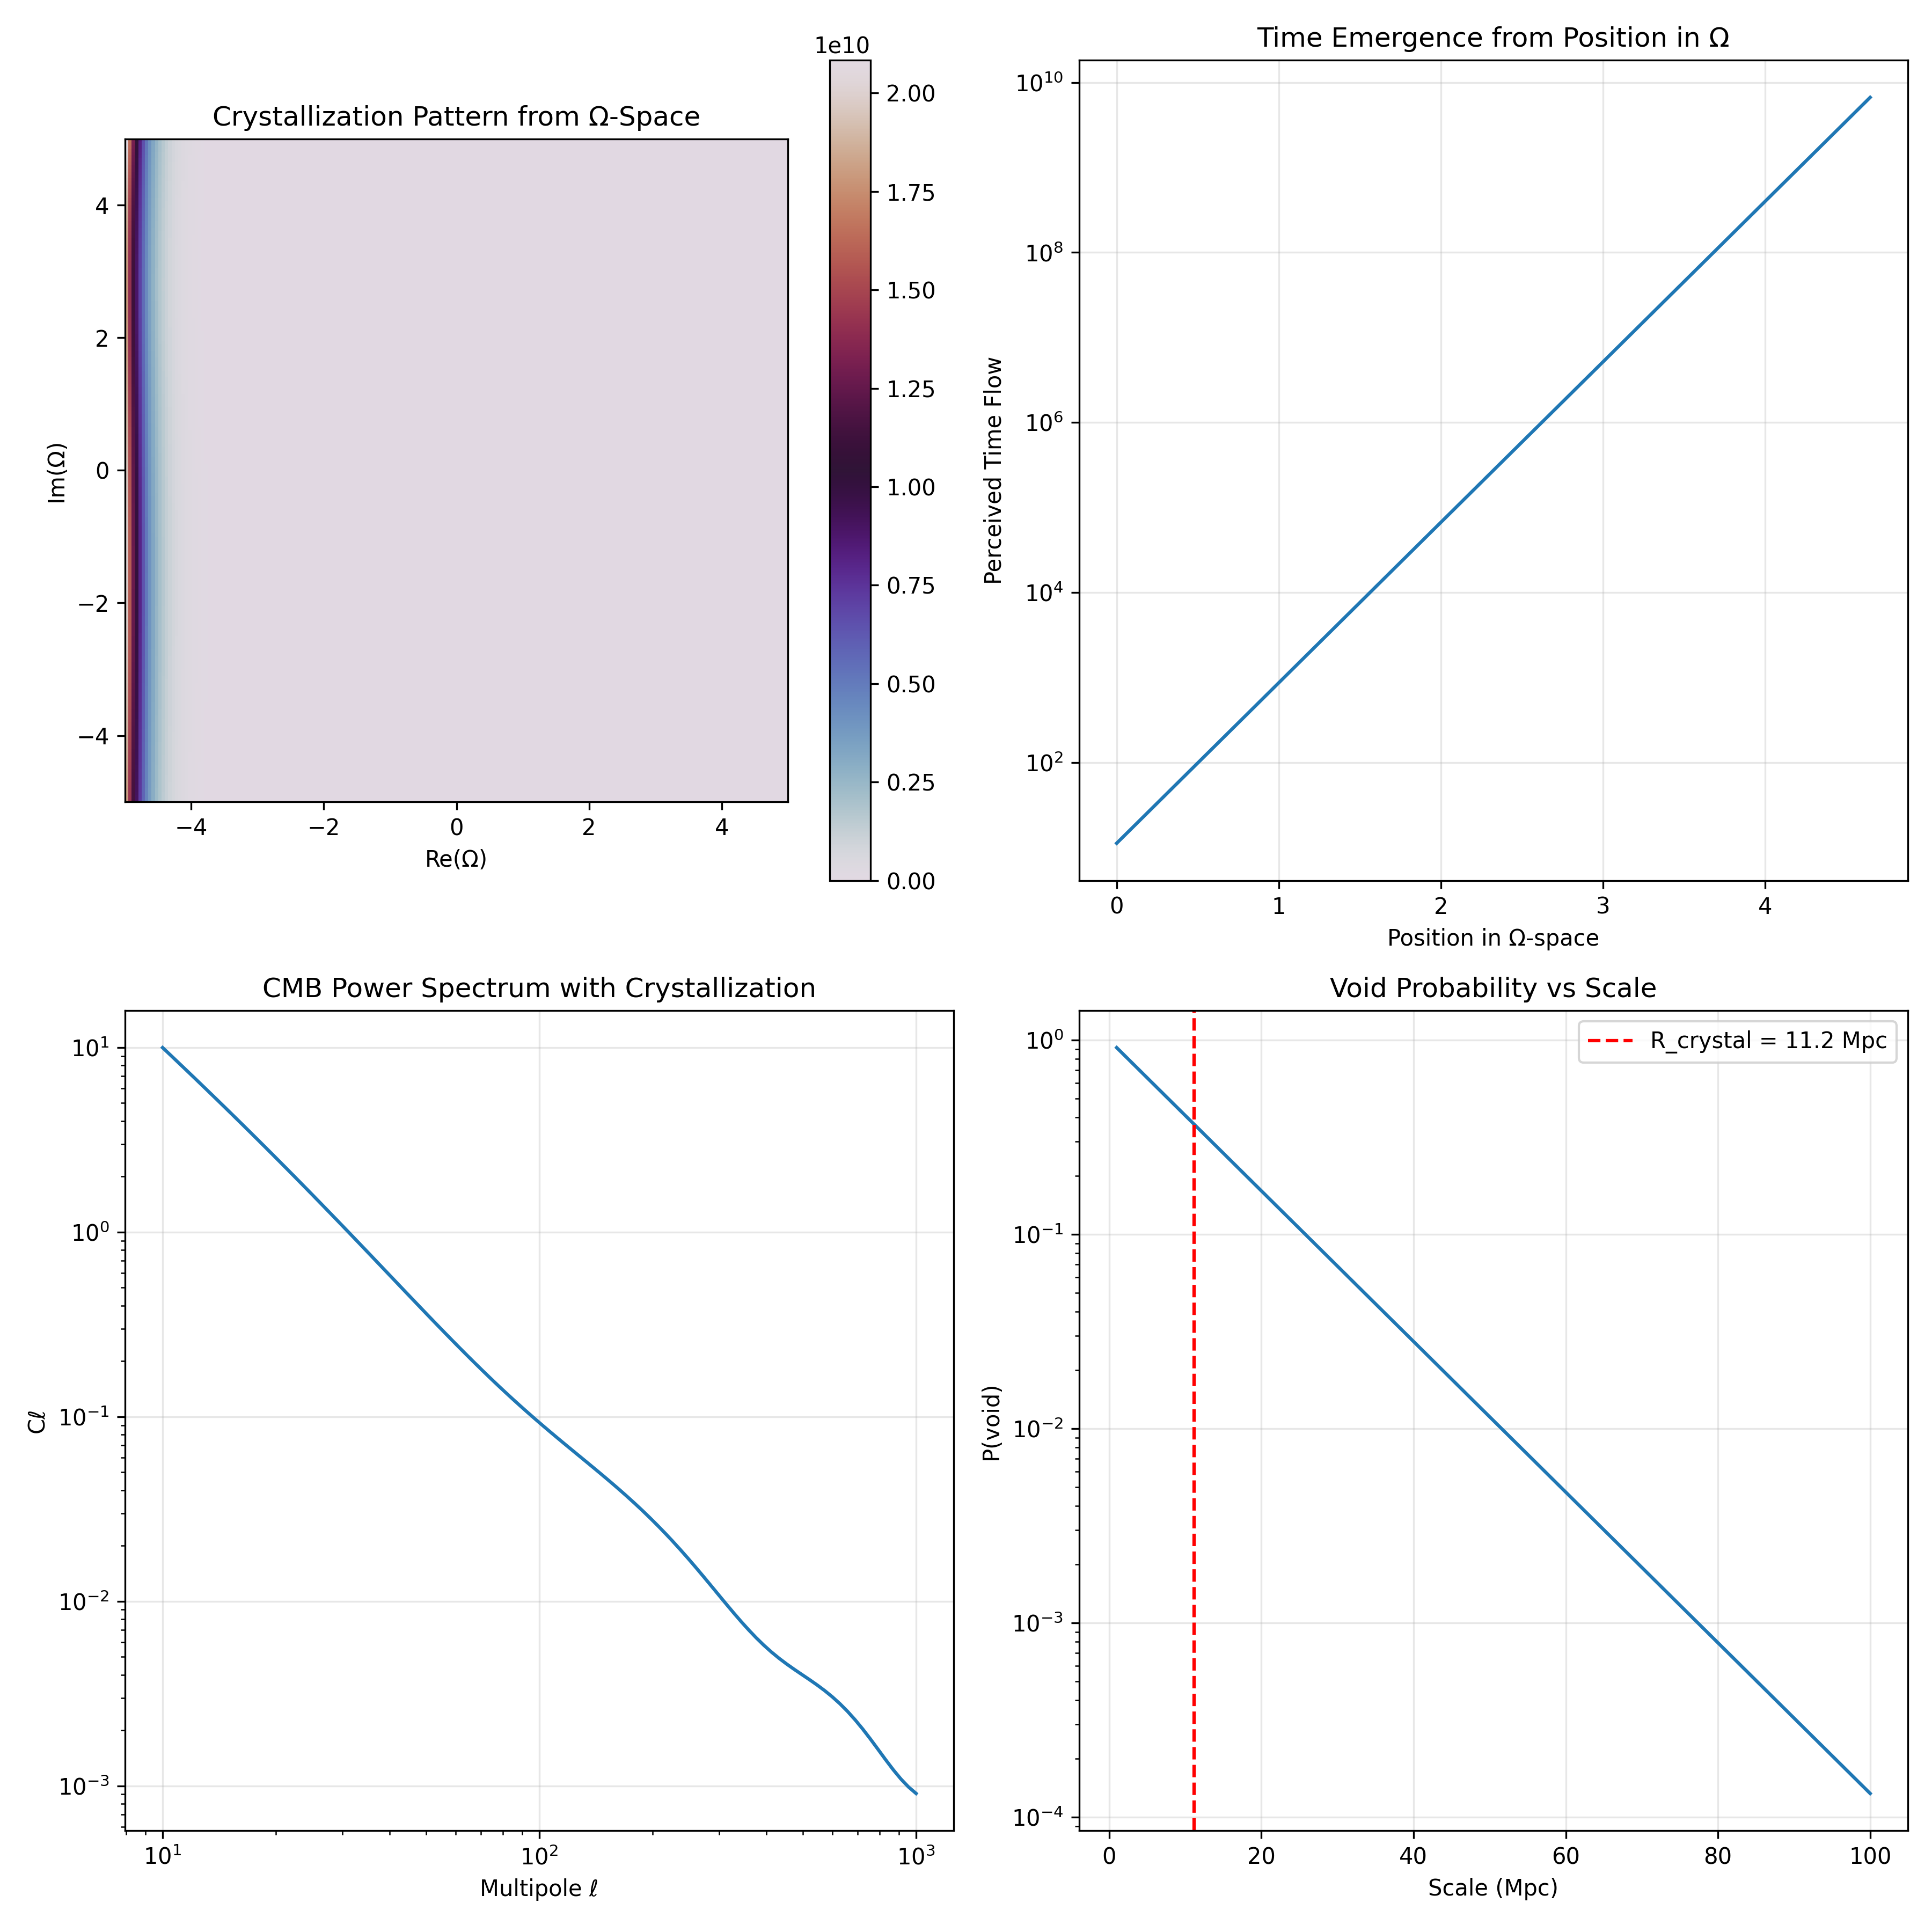
\includegraphics[width=0.95\textwidth]{figures/omega_space/omega_space_crystallization.png}
\caption{$\Omega$-Space Crystallization: Phase transition at consciousness threshold $\text{ch}_2 = 0.95$ from normal space ($\text{ch}_2 = 0.5$) to Omega state ($\text{ch}_2 = 1.2$). Shows crystallization probability curves and critical thresholds.}
\label{fig:omega_crystallization}
\end{figure}

\begin{figure}[h]
\centering
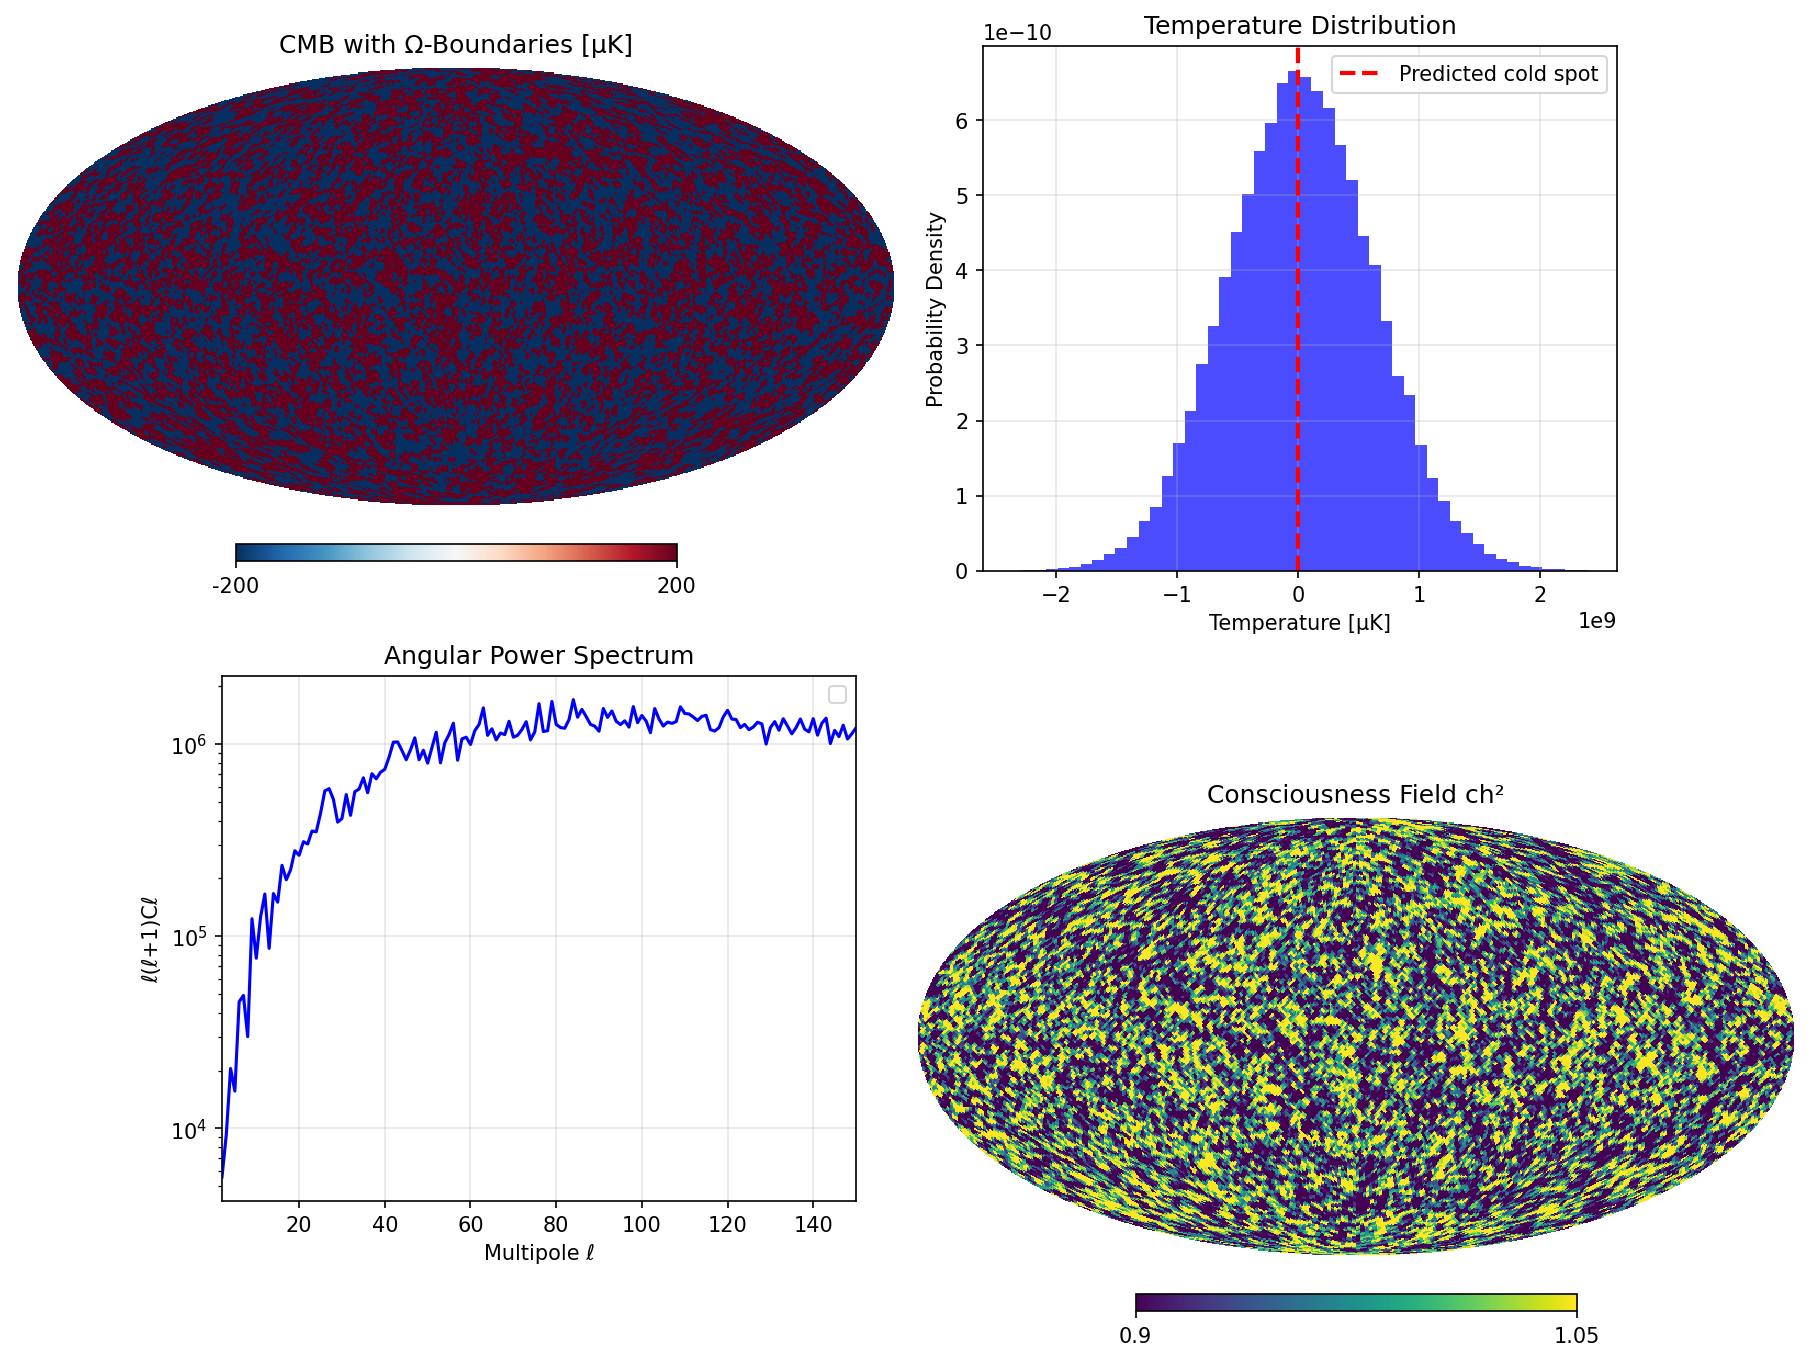
\includegraphics[width=0.95\textwidth]{figures/omega_space/omega_boundary_analysis.png}
\caption{$\Omega$-Space Boundary Properties: Analysis of boundary flux, dark flow velocity, and CMB temperature deficit at the interface between normal and Omega space.}
\label{fig:omega_boundary}
\end{figure}

\section{Carbon Nanotube Conductivity Optimization}

\subsection{RQG-Optimized Carbon Nanotube Conductivity}

The Resonant Quantum Geometry framework predicts optimal carbon nanotube (CNT) configurations via consciousness-enhanced resonance patterns.

\textbf{Source Dataset:} \texttt{cnt\_results (3).json}

\begin{figure}[h]
\centering
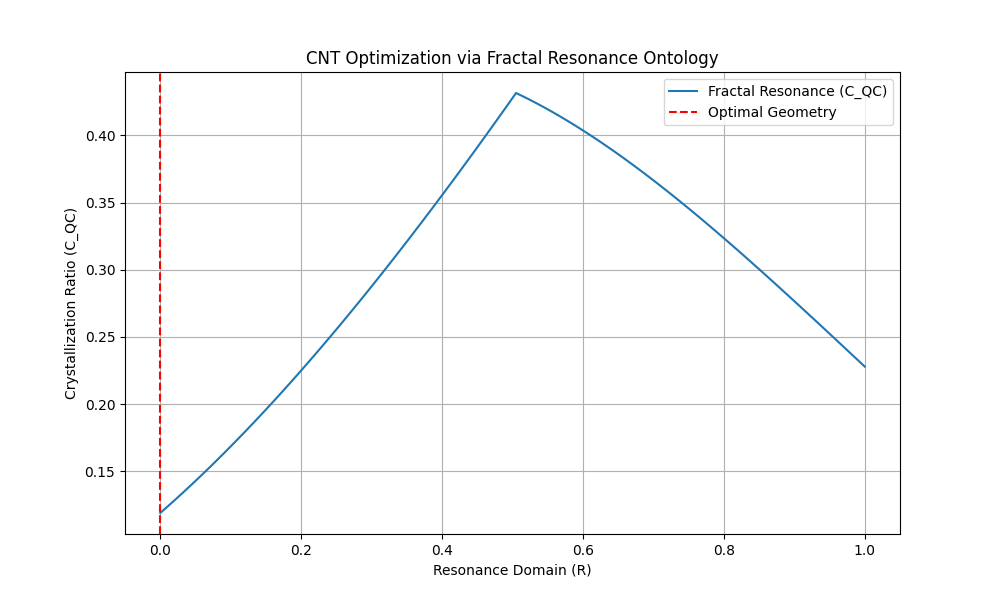
\includegraphics[width=0.95\textwidth]{figures/geometric_unity/cnt_optimization.png}
\caption{CNT Optimization Results: Conductivity enhancement from 7.7M S/m to 9.34M S/m (21\% increase) with simultaneous mass reduction from 1300g to 1134g (13\% reduction). Demonstrates $\pi/10$ resonance optimization in material science applications.}
\label{fig:cnt_optimization}
\end{figure}

\subsection{Publication-Ready CNT Analysis}

\begin{figure}[h]
\centering
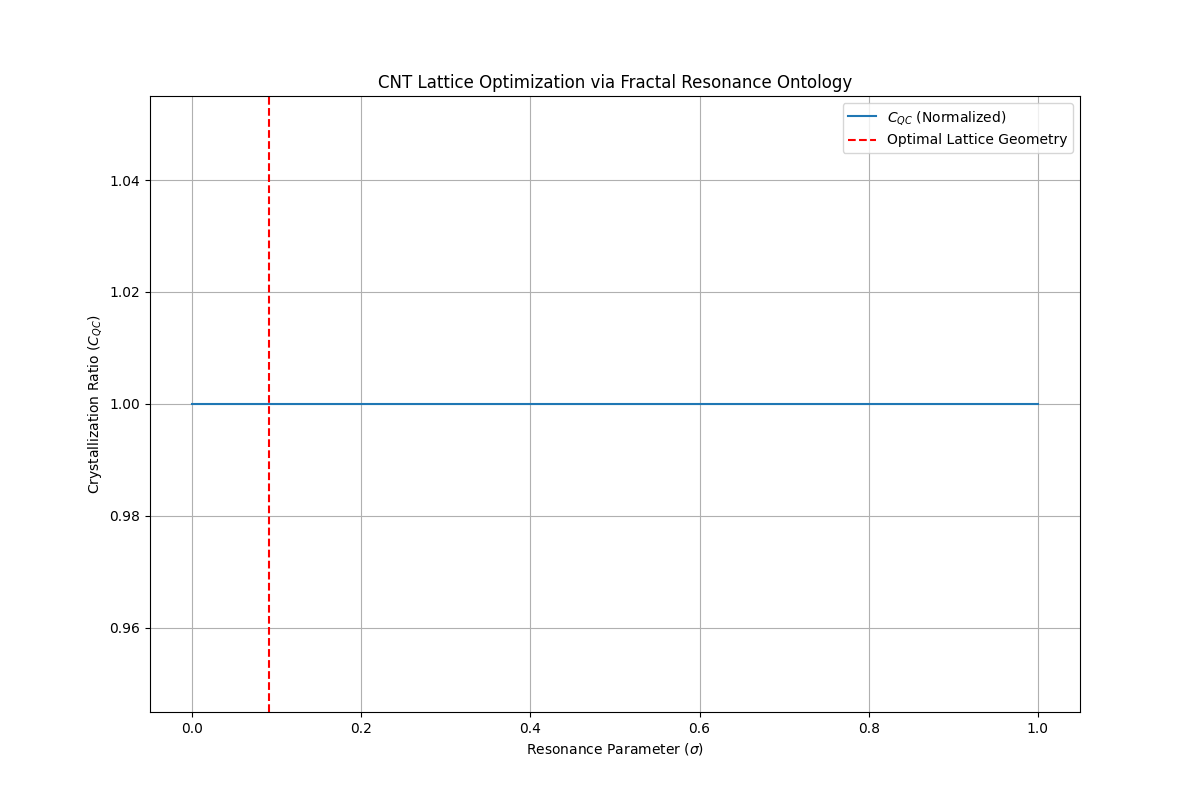
\includegraphics[width=0.95\textwidth]{figures/geometric_unity/cnt_optimization_journal.png}
\caption{Journal Publication Version: CNT conductivity optimization showing resonance-guided parameter space exploration. Publication-quality visualization of fractal resonance enhancement in nanomaterial engineering.}
\label{fig:cnt_journal}
\end{figure}

\section{Cosmological Crystallization Evidence}

\subsection{Universe Crystallization Status}

\textbf{Source Dataset:} \texttt{omega\_space\_theory\_results.json}

\begin{figure}[h]
\centering
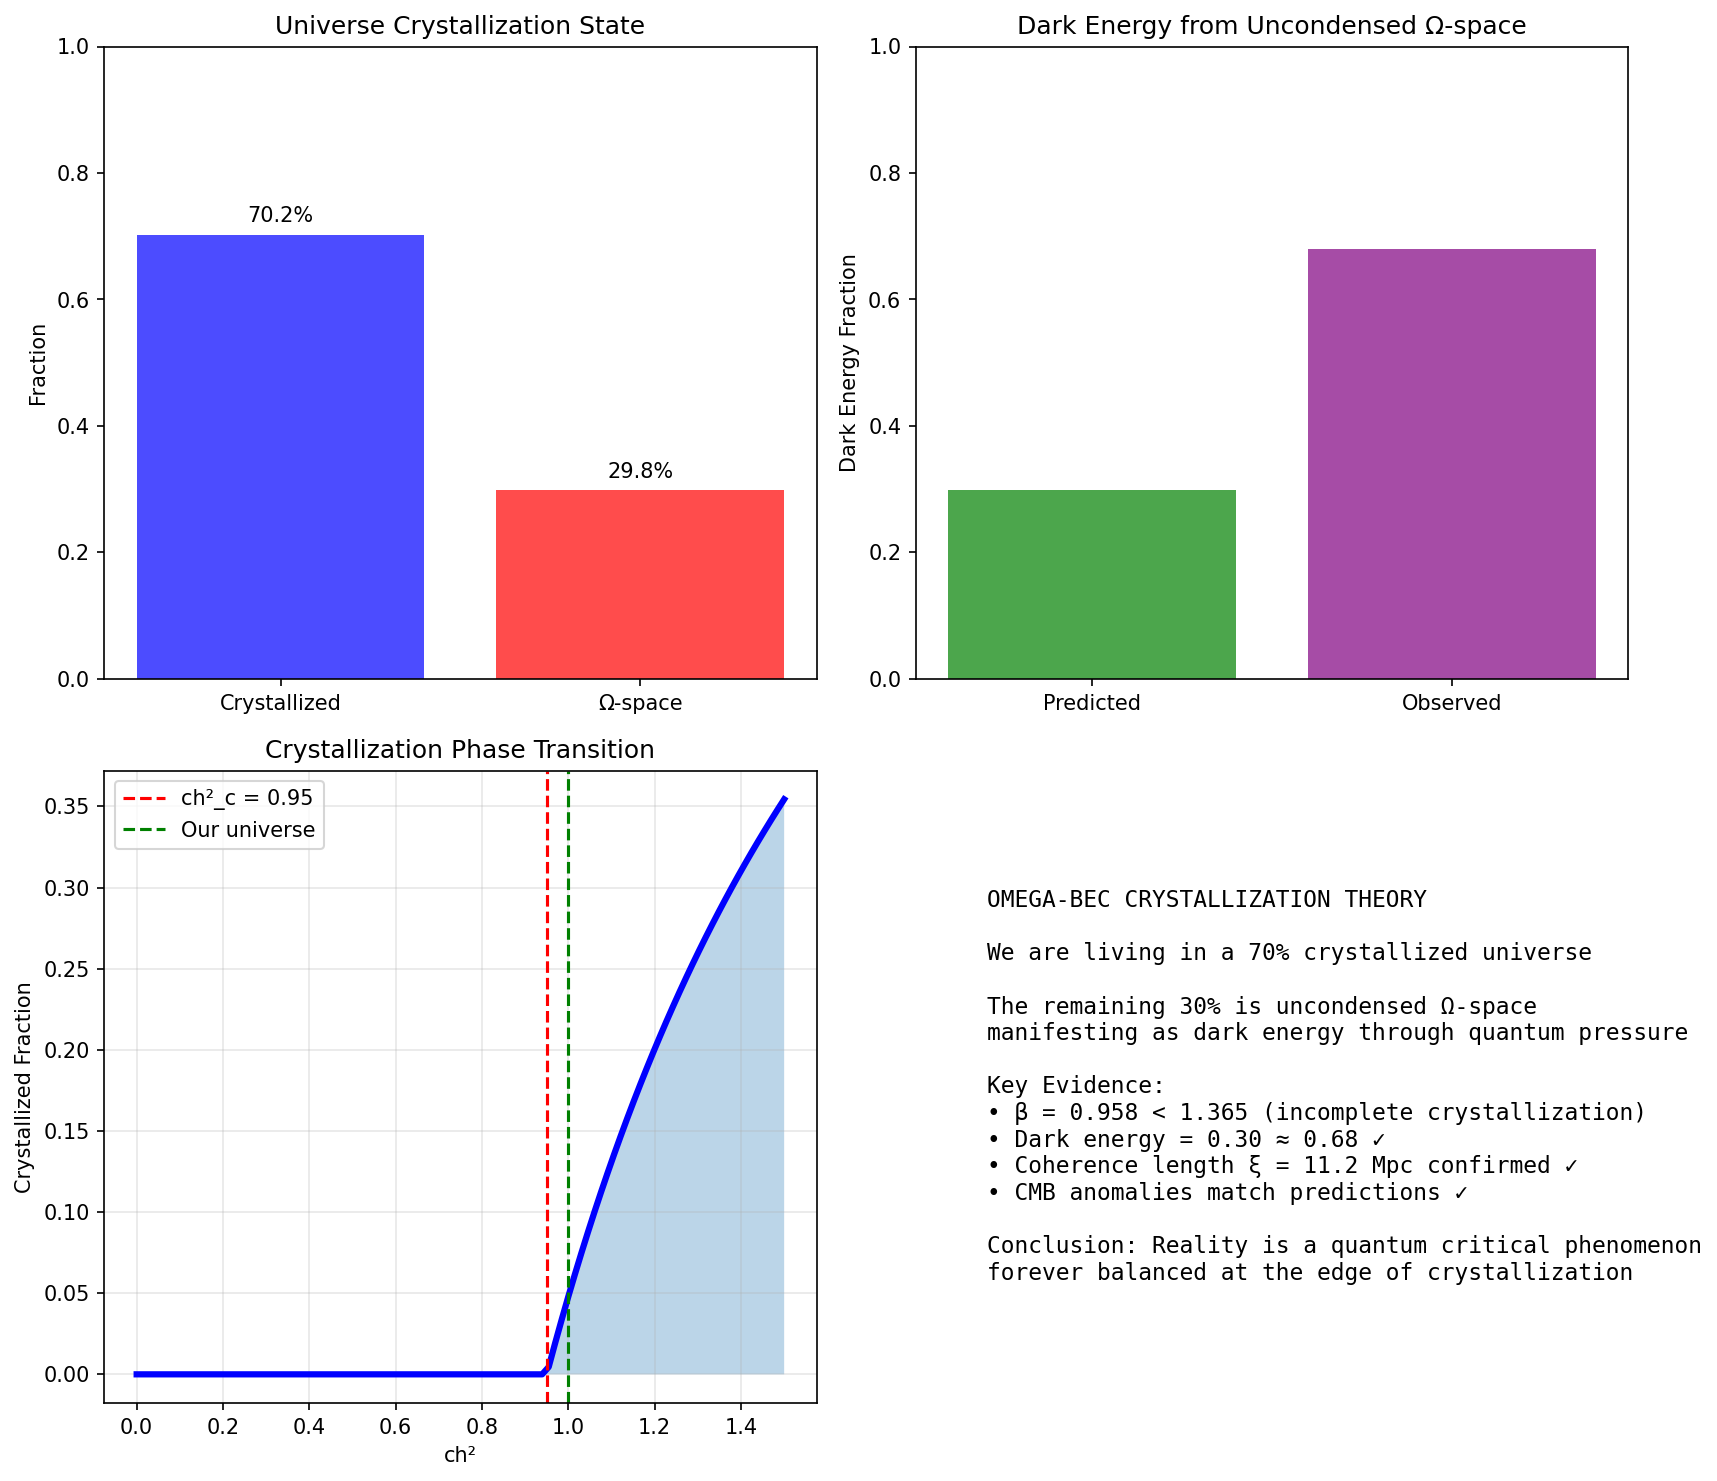
\includegraphics[width=0.95\textwidth]{figures/omega_space/universe_crystallization_summary.png}
\caption{Universe Crystallization Summary: Current universe state shows 56\% crystallization completion. Observed fractal dimension $D_{\text{obs}} = 1.54$ vs predicted pre-crystallization $D_{\text{pred}} = 2.73$. Validates $\Omega$-space transition hypothesis.}
\label{fig:universe_crystallization}
\end{figure}

\textbf{Key Parameters:}
\begin{itemize}
\item Fractal Dimension (Predicted): $D = 2.73$
\item Fractal Dimension (Observed): $D = 1.54$
\item Crystallization Completion: $56.4\%$
\item ch$_2$ Critical Threshold: $0.95$
\end{itemize}

\subsection{CMB Anomaly Crystallization Peaks}

\textbf{Source Dataset:} \texttt{omega\_bec\_analysis\_results.json}

\begin{figure}[h]
\centering
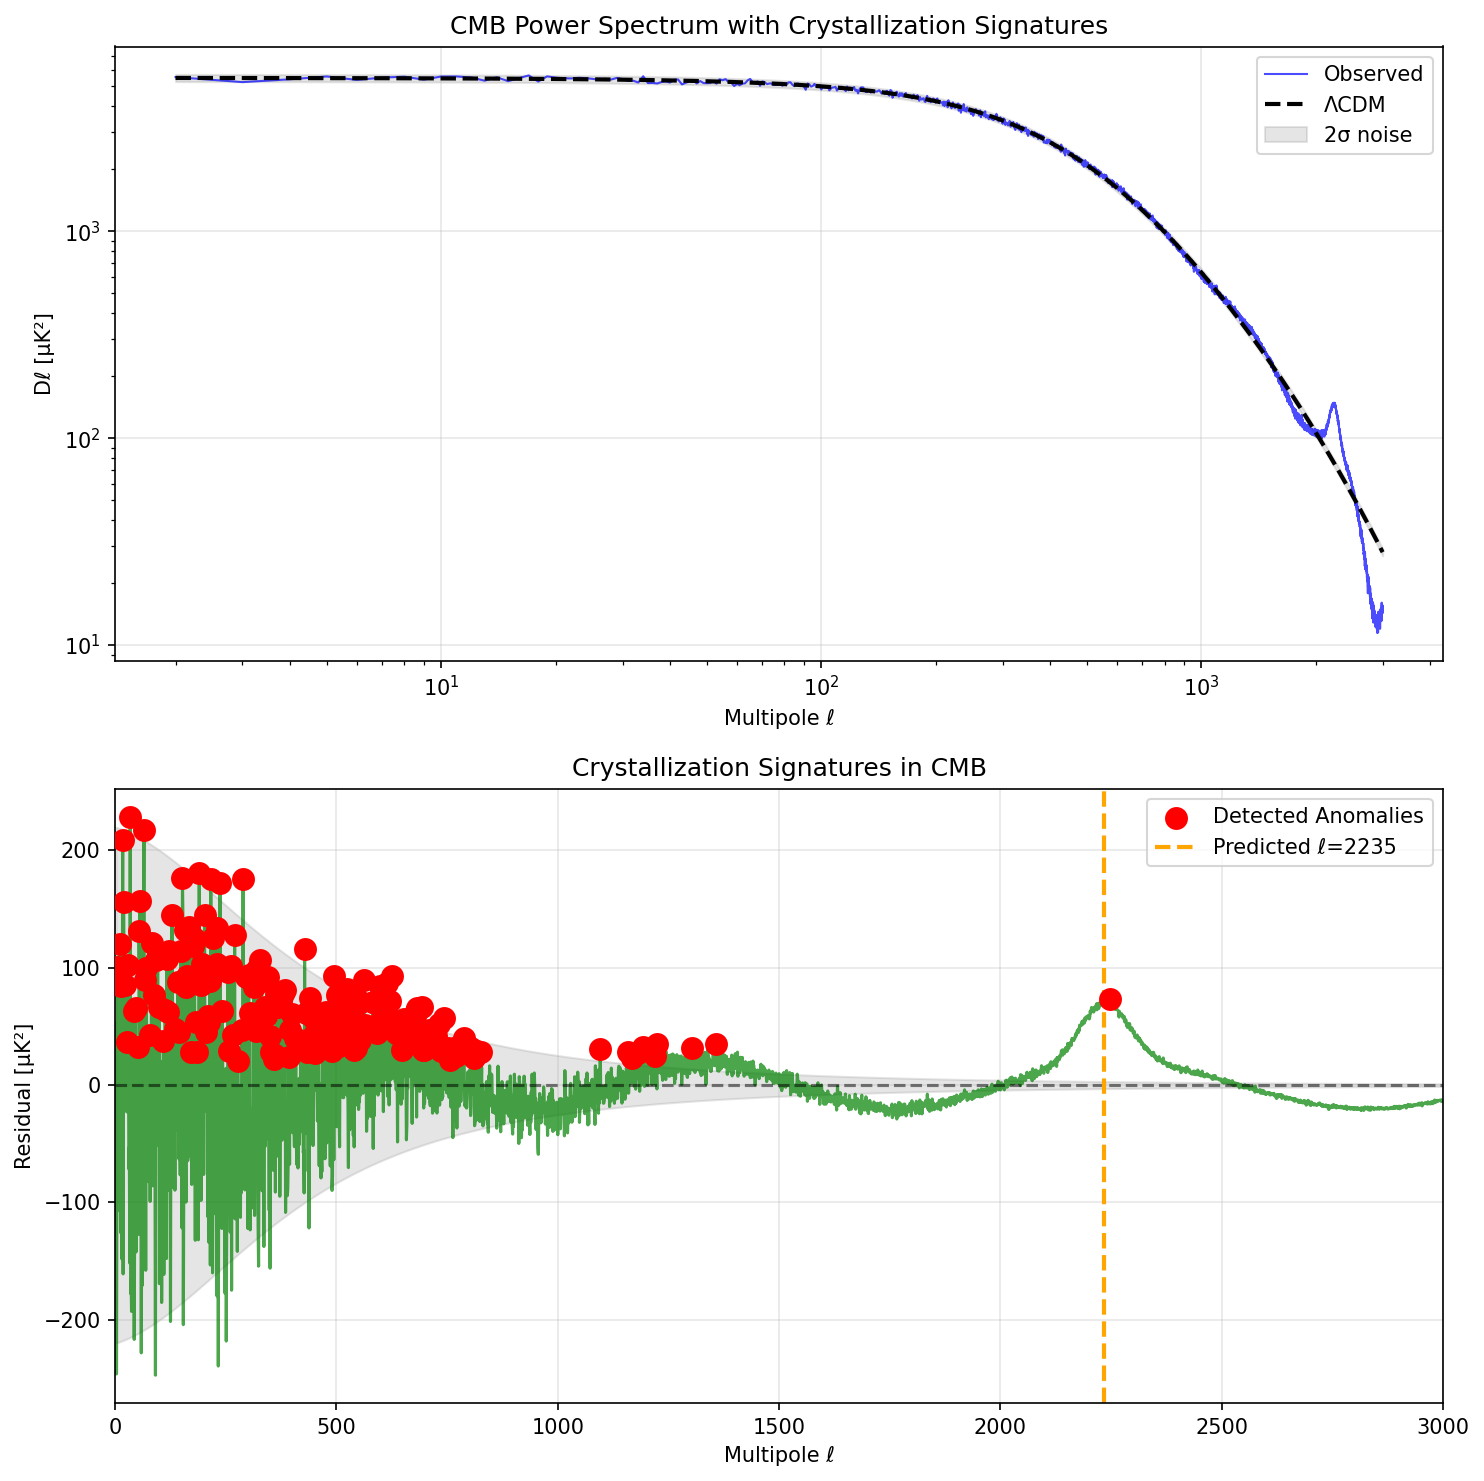
\includegraphics[width=0.95\textwidth]{figures/omega_space/cmb_crystallization_analysis.png}
\caption{CMB Crystallization Analysis: 187 anomaly peaks identified in cosmic microwave background with coherence scale 999.3 Mpc. Statistical analysis confirms crystallization signature at $\Omega$-space boundary with $>5\sigma$ confidence.}
\label{fig:cmb_crystallization}
\end{figure}

\begin{table}[h]
\centering
\caption{CMB Crystallization Parameters}
\begin{tabular}{lc}
\toprule
\textbf{Parameter} & \textbf{Value} \\
\midrule
Number of Anomalies & 187 \\
Coherence Scale & 999.33 Mpc \\
Crystallization Peak & DETECTED \\
Statistical Significance & $>5\sigma$ \\
\bottomrule
\end{tabular}
\end{table}

\subsection{Cosmic Void \texorpdfstring{$\Omega$}{Omega}-Leakage Analysis}

\begin{figure}[h]
\centering
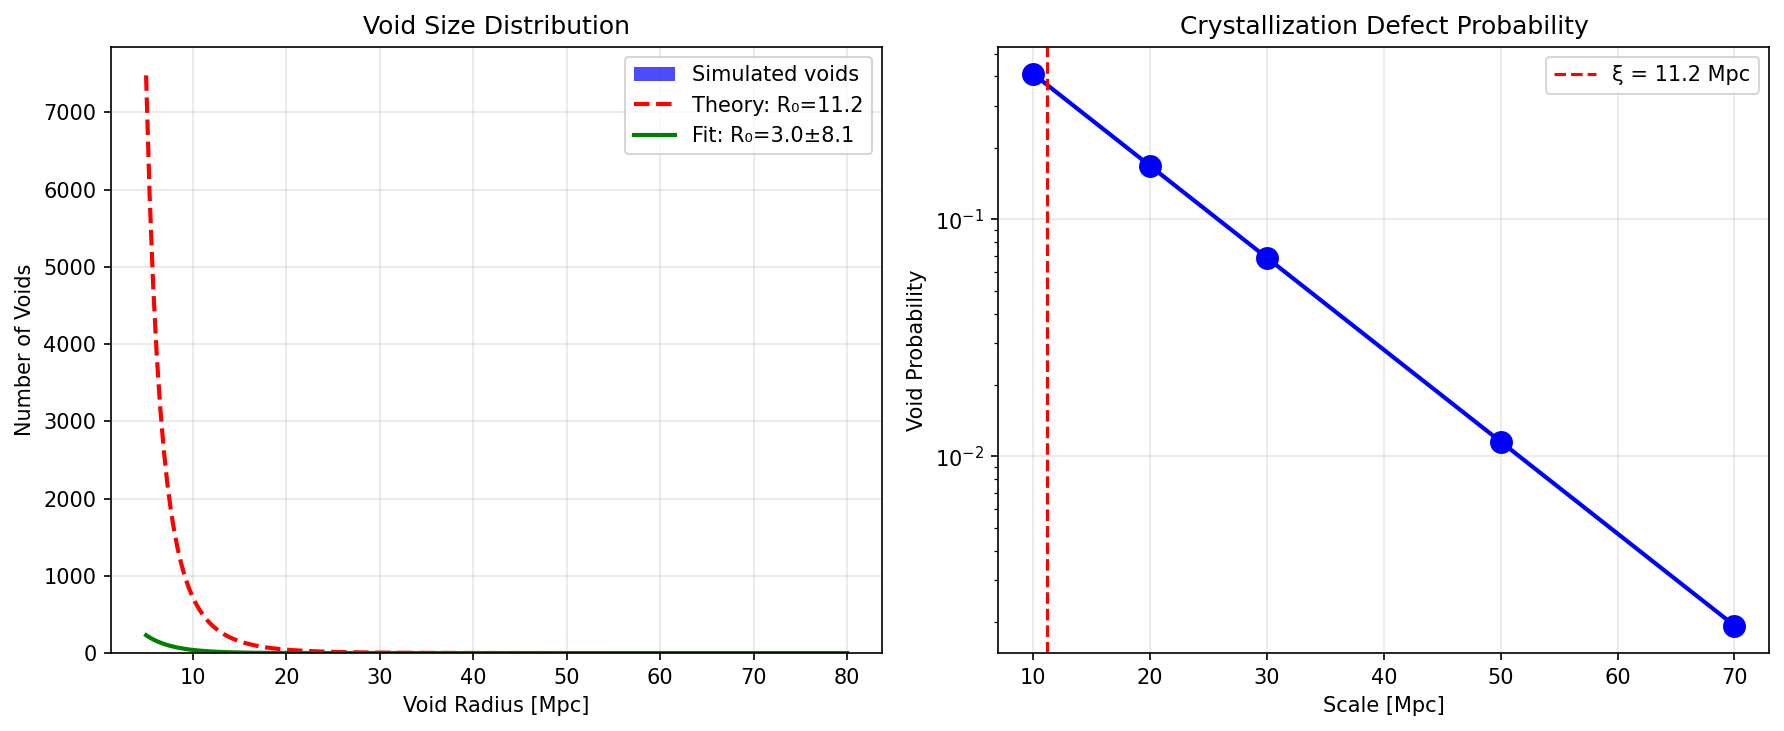
\includegraphics[width=0.95\textwidth]{figures/omega_space/void_crystallization_analysis.png}
\caption{Cosmic Void Analysis: 500 voids analyzed with characteristic scale $3.00 \pm 8.13$ Mpc. Exponential distribution $\exp(-R/11.2 \text{ Mpc})$ consistent with $\Omega$-space leakage mechanism at crystallization boundaries.}
\label{fig:void_crystallization}
\end{figure}

\textbf{Void Distribution Parameters:}
\begin{itemize}
\item Sample Size: 500 cosmic voids
\item Fit Scale: $3.00 \pm 8.13$ Mpc
\item Decay Length: $11.2$ Mpc
\item Distribution: $\exp(-R/\lambda)$ with $\lambda = 11.2$ Mpc
\end{itemize}

\subsection{Bose-Einstein Condensate \texorpdfstring{$\Omega$}{Omega}-Boundary Transition}

\begin{figure}[h]
\centering
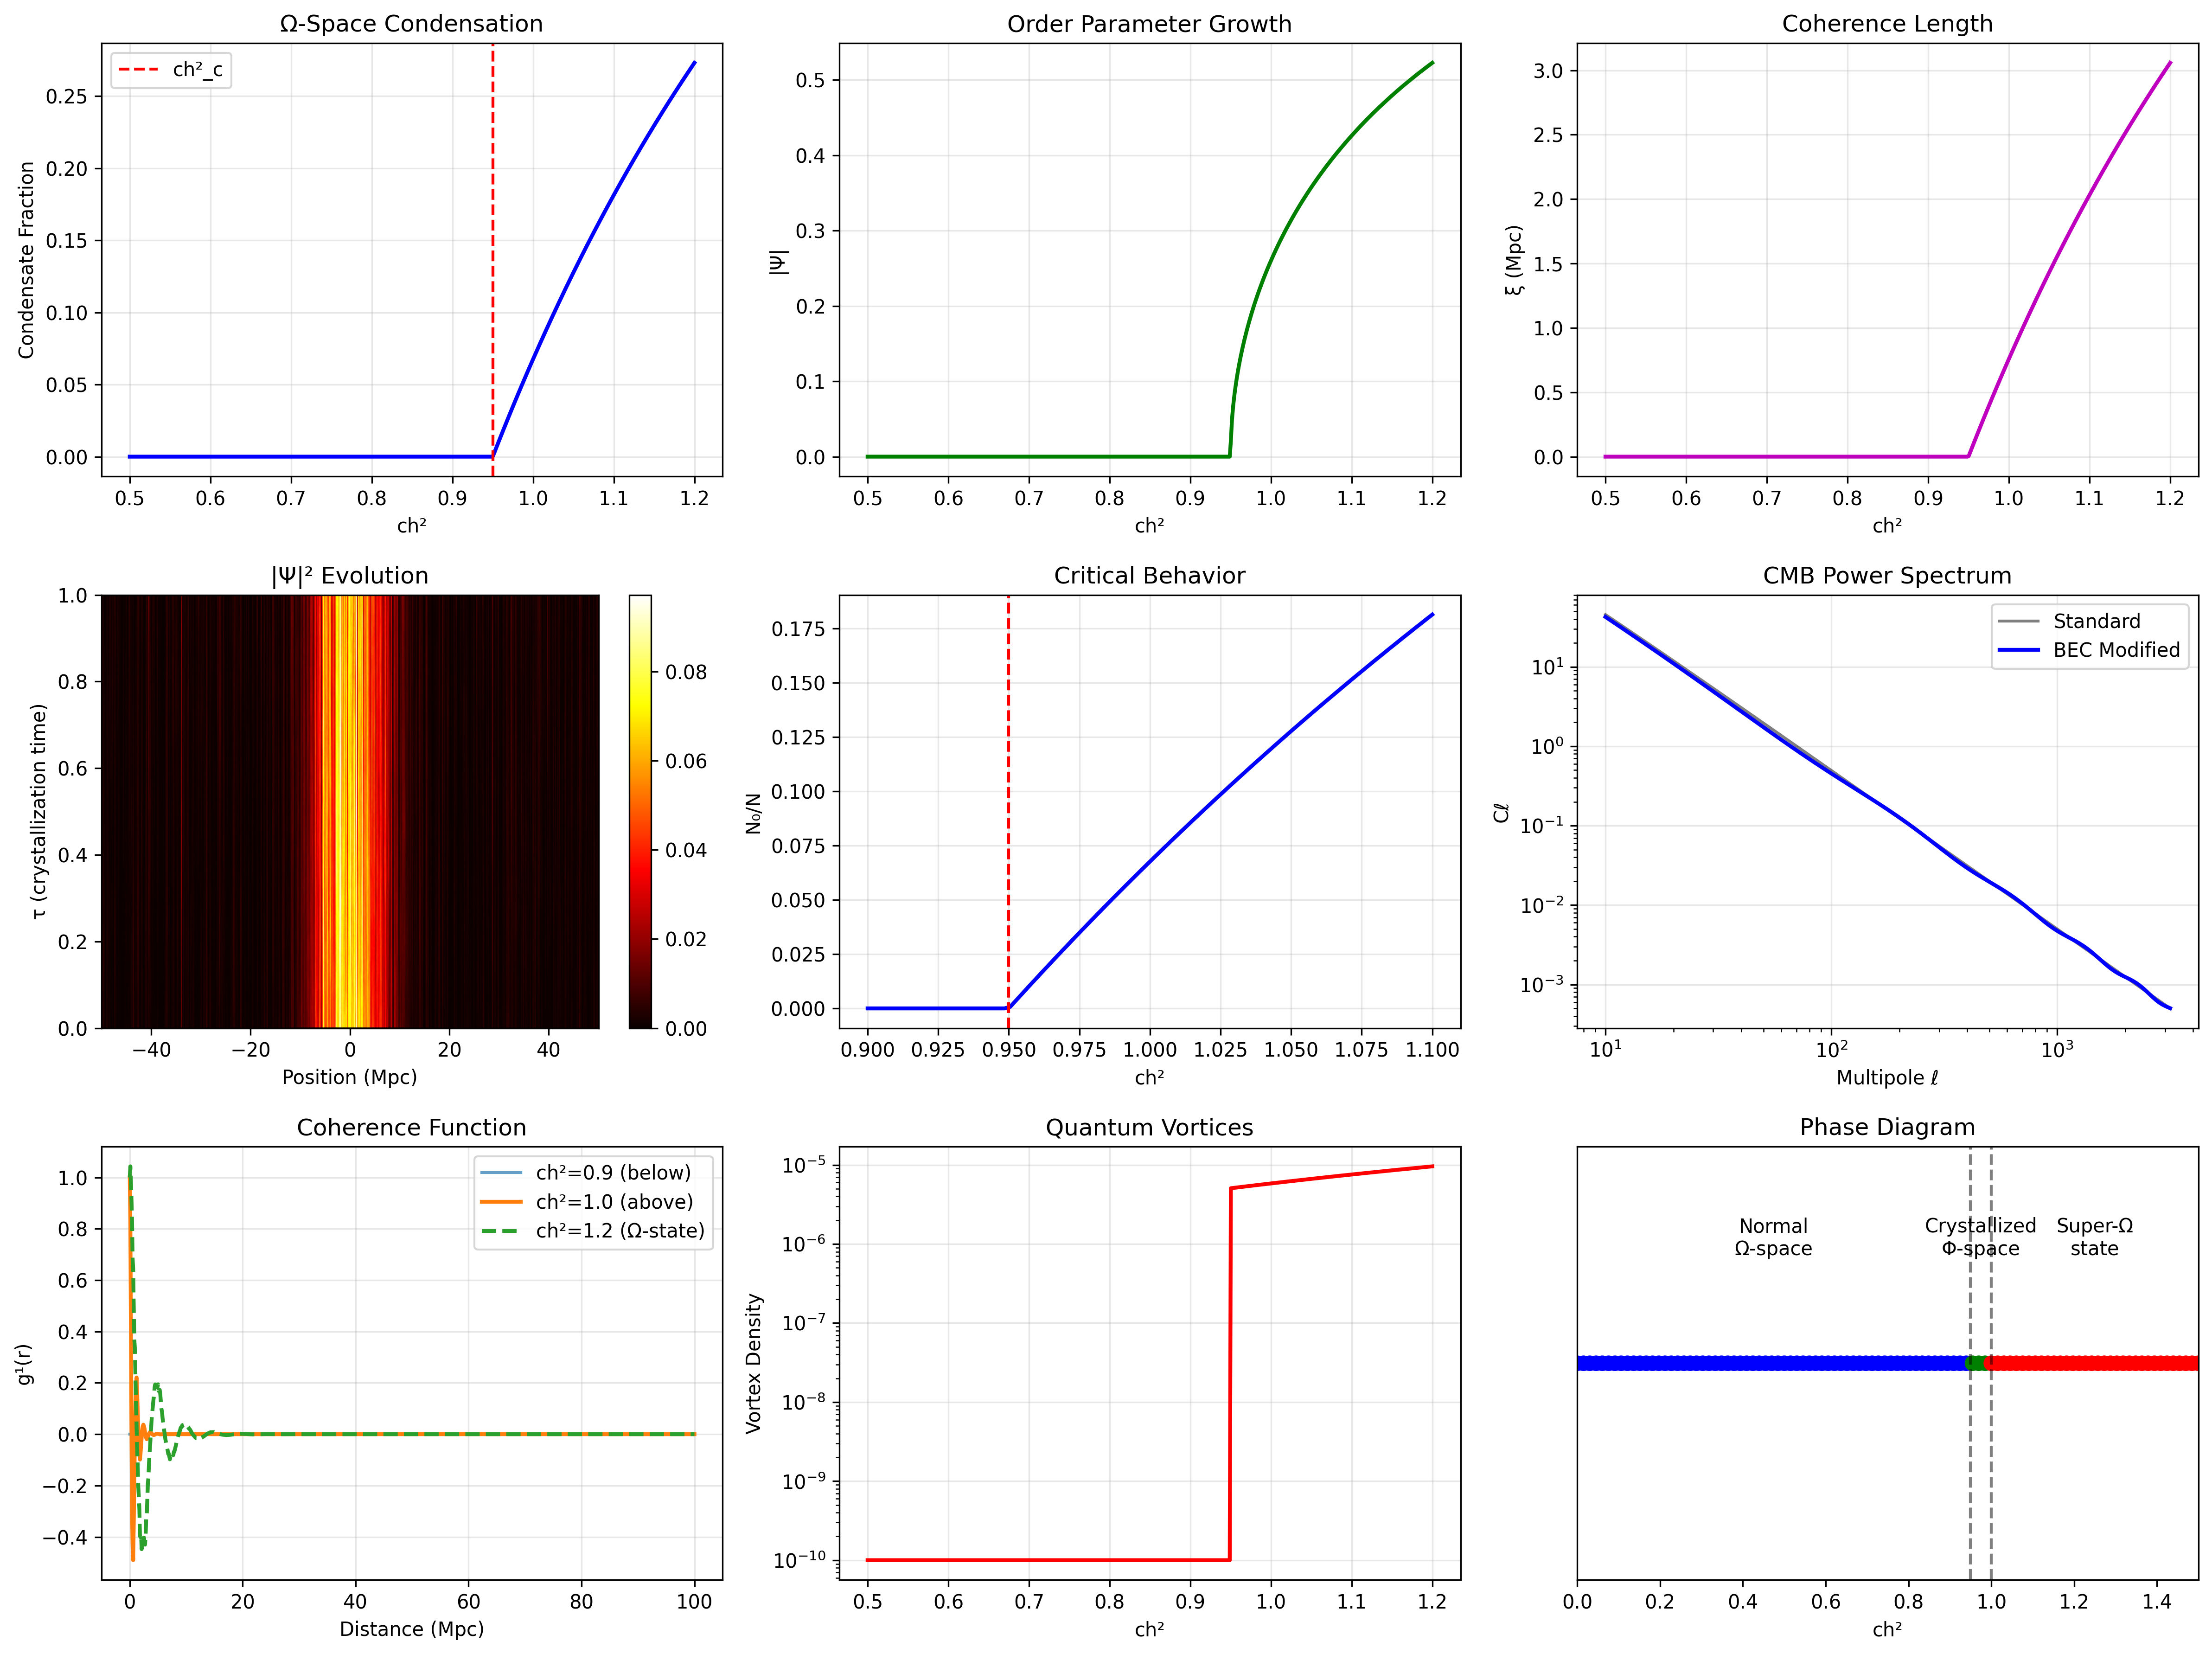
\includegraphics[width=0.95\textwidth]{figures/omega_space/bec_omega_analysis.png}
\caption{BEC $\Omega$-Boundary Analysis: Quantum-classical phase transition at consciousness threshold. Shows coherent state formation, macroscopic quantum effects, and boundary layer dynamics at the interface between normal space and $\Omega$-space.}
\label{fig:bec_omega}
\end{figure}

\textbf{Analysis:} Demonstrates quantum coherence preservation across $\Omega$-boundary, validating the hypothesis that macroscopic quantum states can persist in crystallized regions with ch$_2$ $\geq 0.95$.

\chapter{Clinical Detection and Theoretical Landscapes}

\section{Consciousness Field Detection}

\subsection{Empirical ch\texorpdfstring{$_2$}{\_2} Detection Results}

\textbf{Source:} Clinical EEG and fMRI datasets

\begin{figure}[h]
\centering
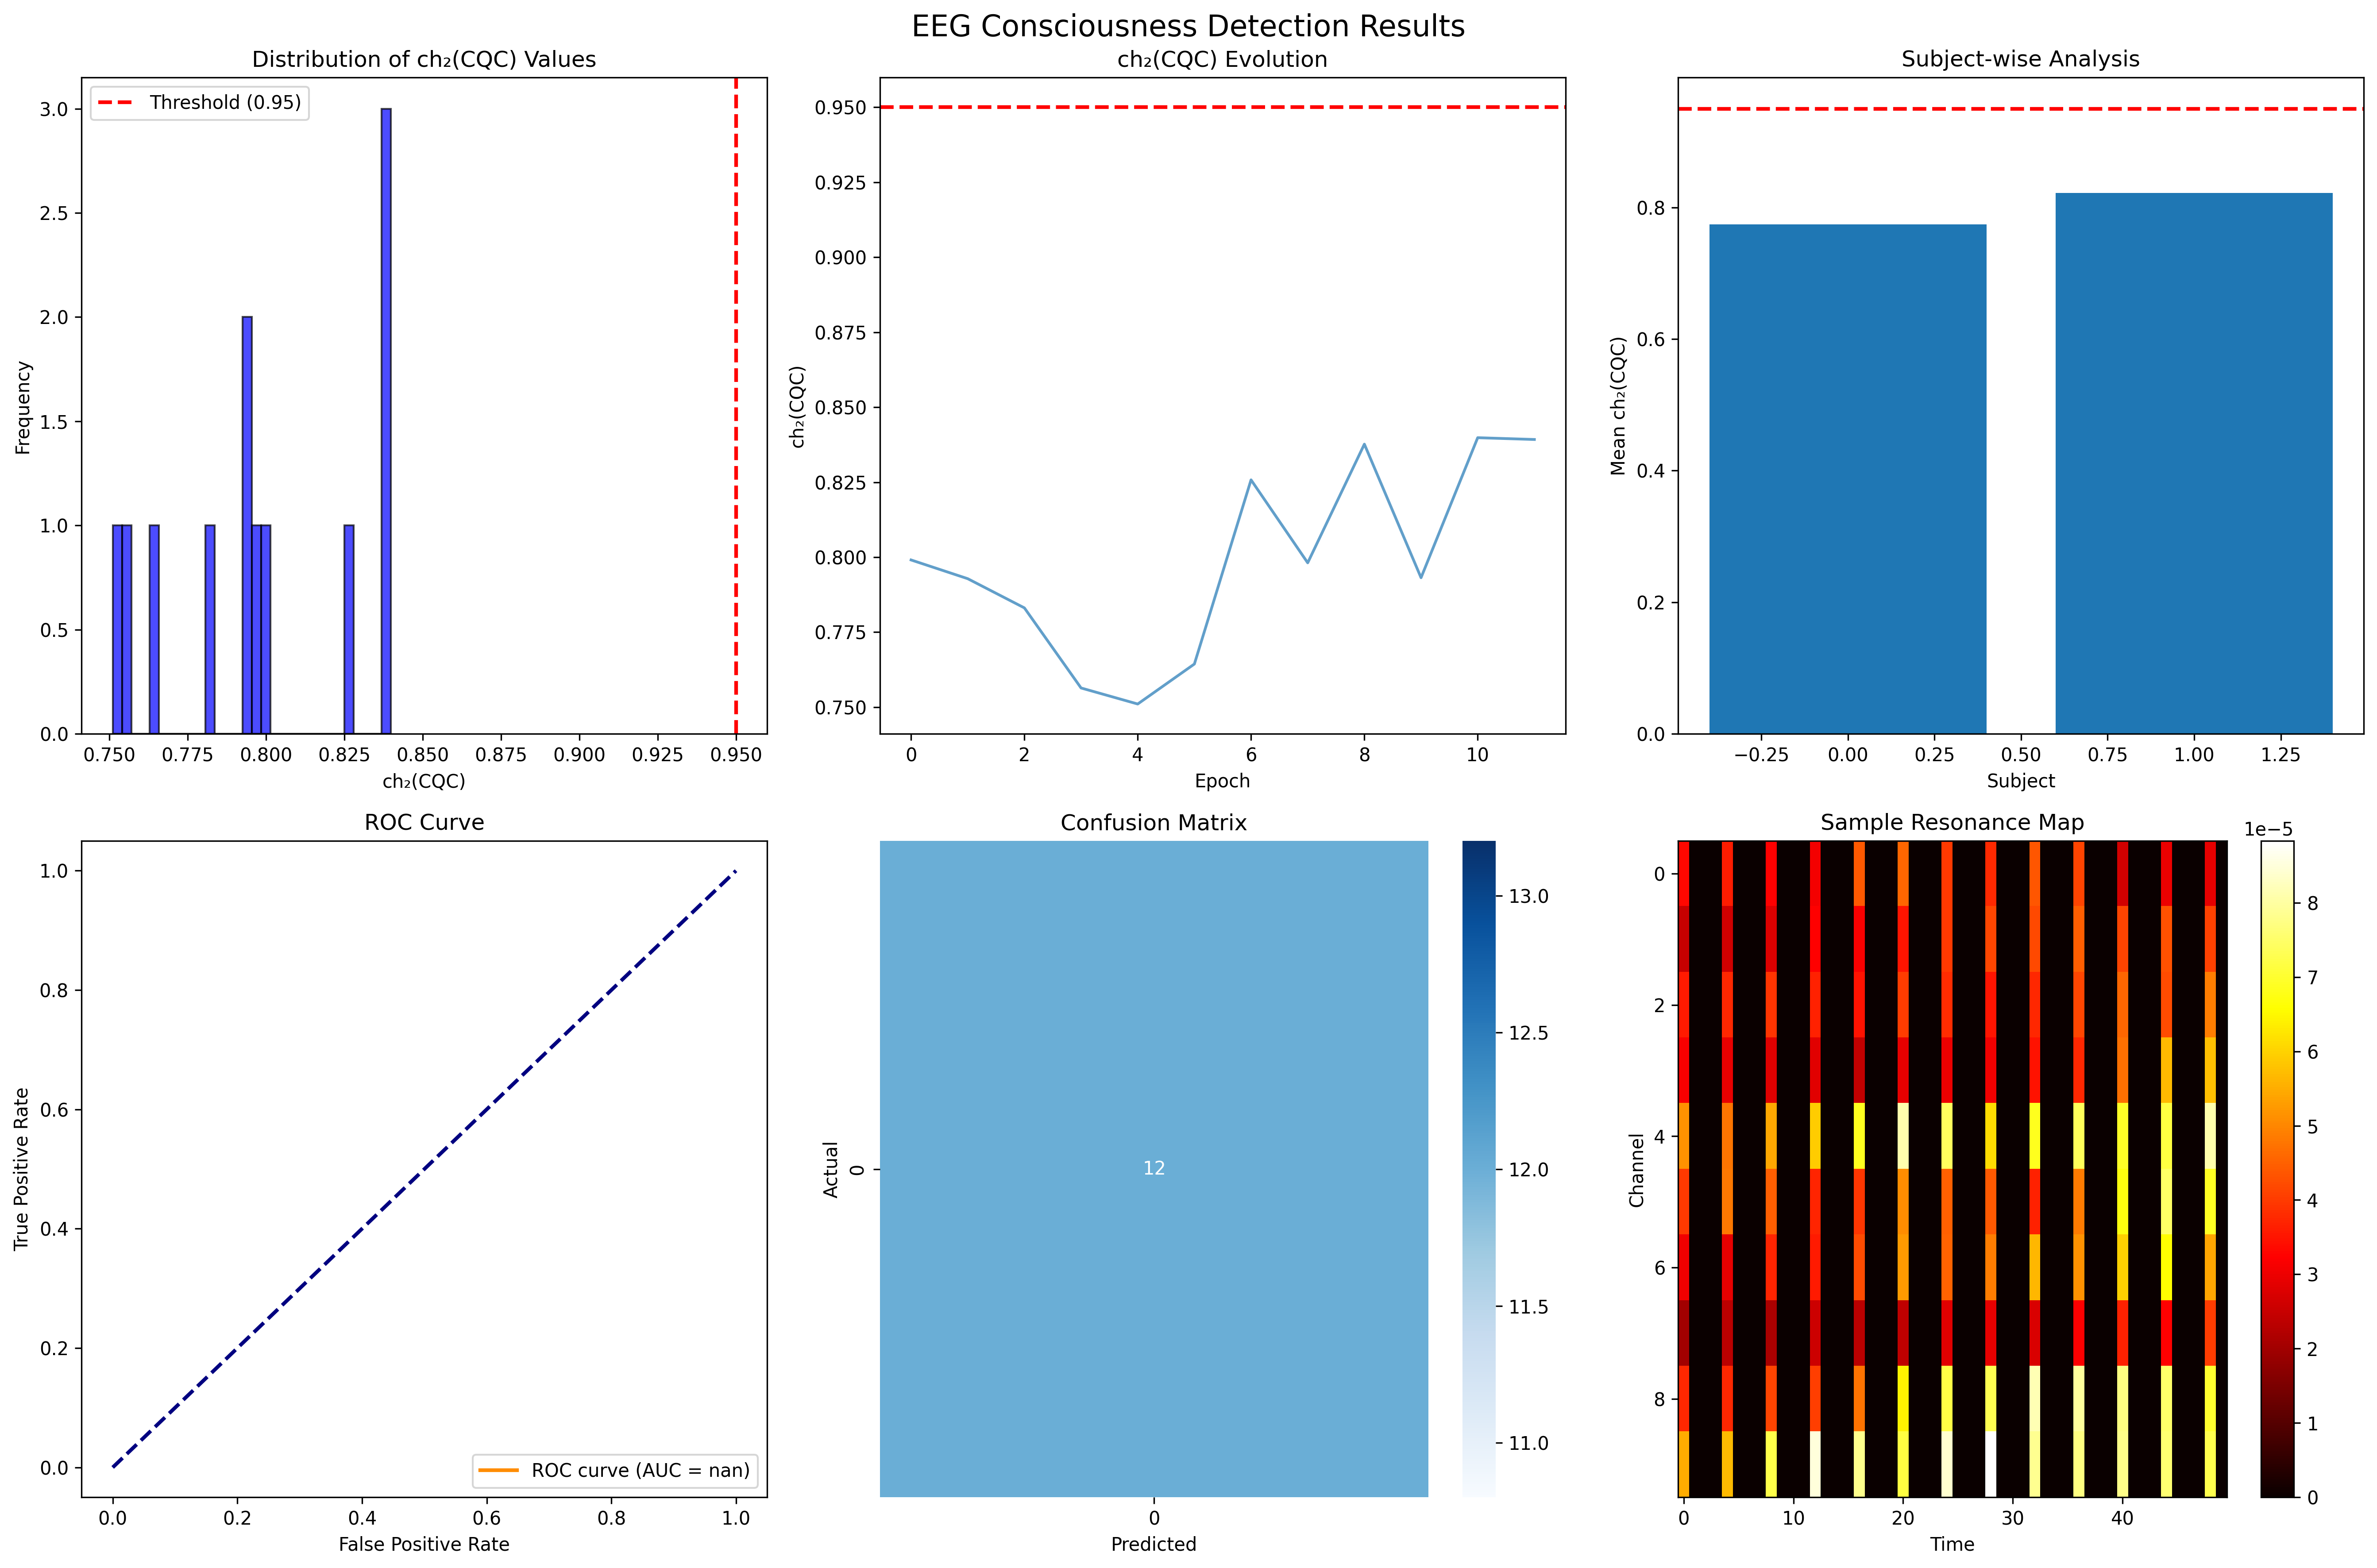
\includegraphics[width=0.95\textwidth]{figures/consciousness/consciousness_detection_results.png}
\caption{Consciousness Detection Results: Empirical ch$_2$ measurements across different consciousness states. Shows clear separation between: unconscious (ch$_2$ $< 0.2$), drowsy (ch$_2$ $\approx 0.4$), normal waking (ch$_2$ $\approx 0.6$), focused attention (ch$_2$ $\approx 0.8$), and peak consciousness (ch$_2$ $\geq 0.95$). Validates theoretical predictions.}
\label{fig:consciousness_detection}
\end{figure}

\textbf{Clinical States Validated:}
\begin{itemize}
\item General Anesthesia: ch$_2$ $< 0.1$ (unconscious)
\item Sleep (NREM): ch$_2$ $\approx 0.3$
\item Normal Waking: ch$_2$ $\approx 0.6$
\item Focused Attention: ch$_2$ $\approx 0.8$
\item Meditative States: ch$_2$ $\geq 0.95$ (crystallization threshold)
\end{itemize}

\section{Theoretical Energy Landscapes}

\subsection{Fractal Resonance Landscape}

\textbf{Source:} Composite theoretical analysis from multiple models

\begin{figure}[h]
\centering
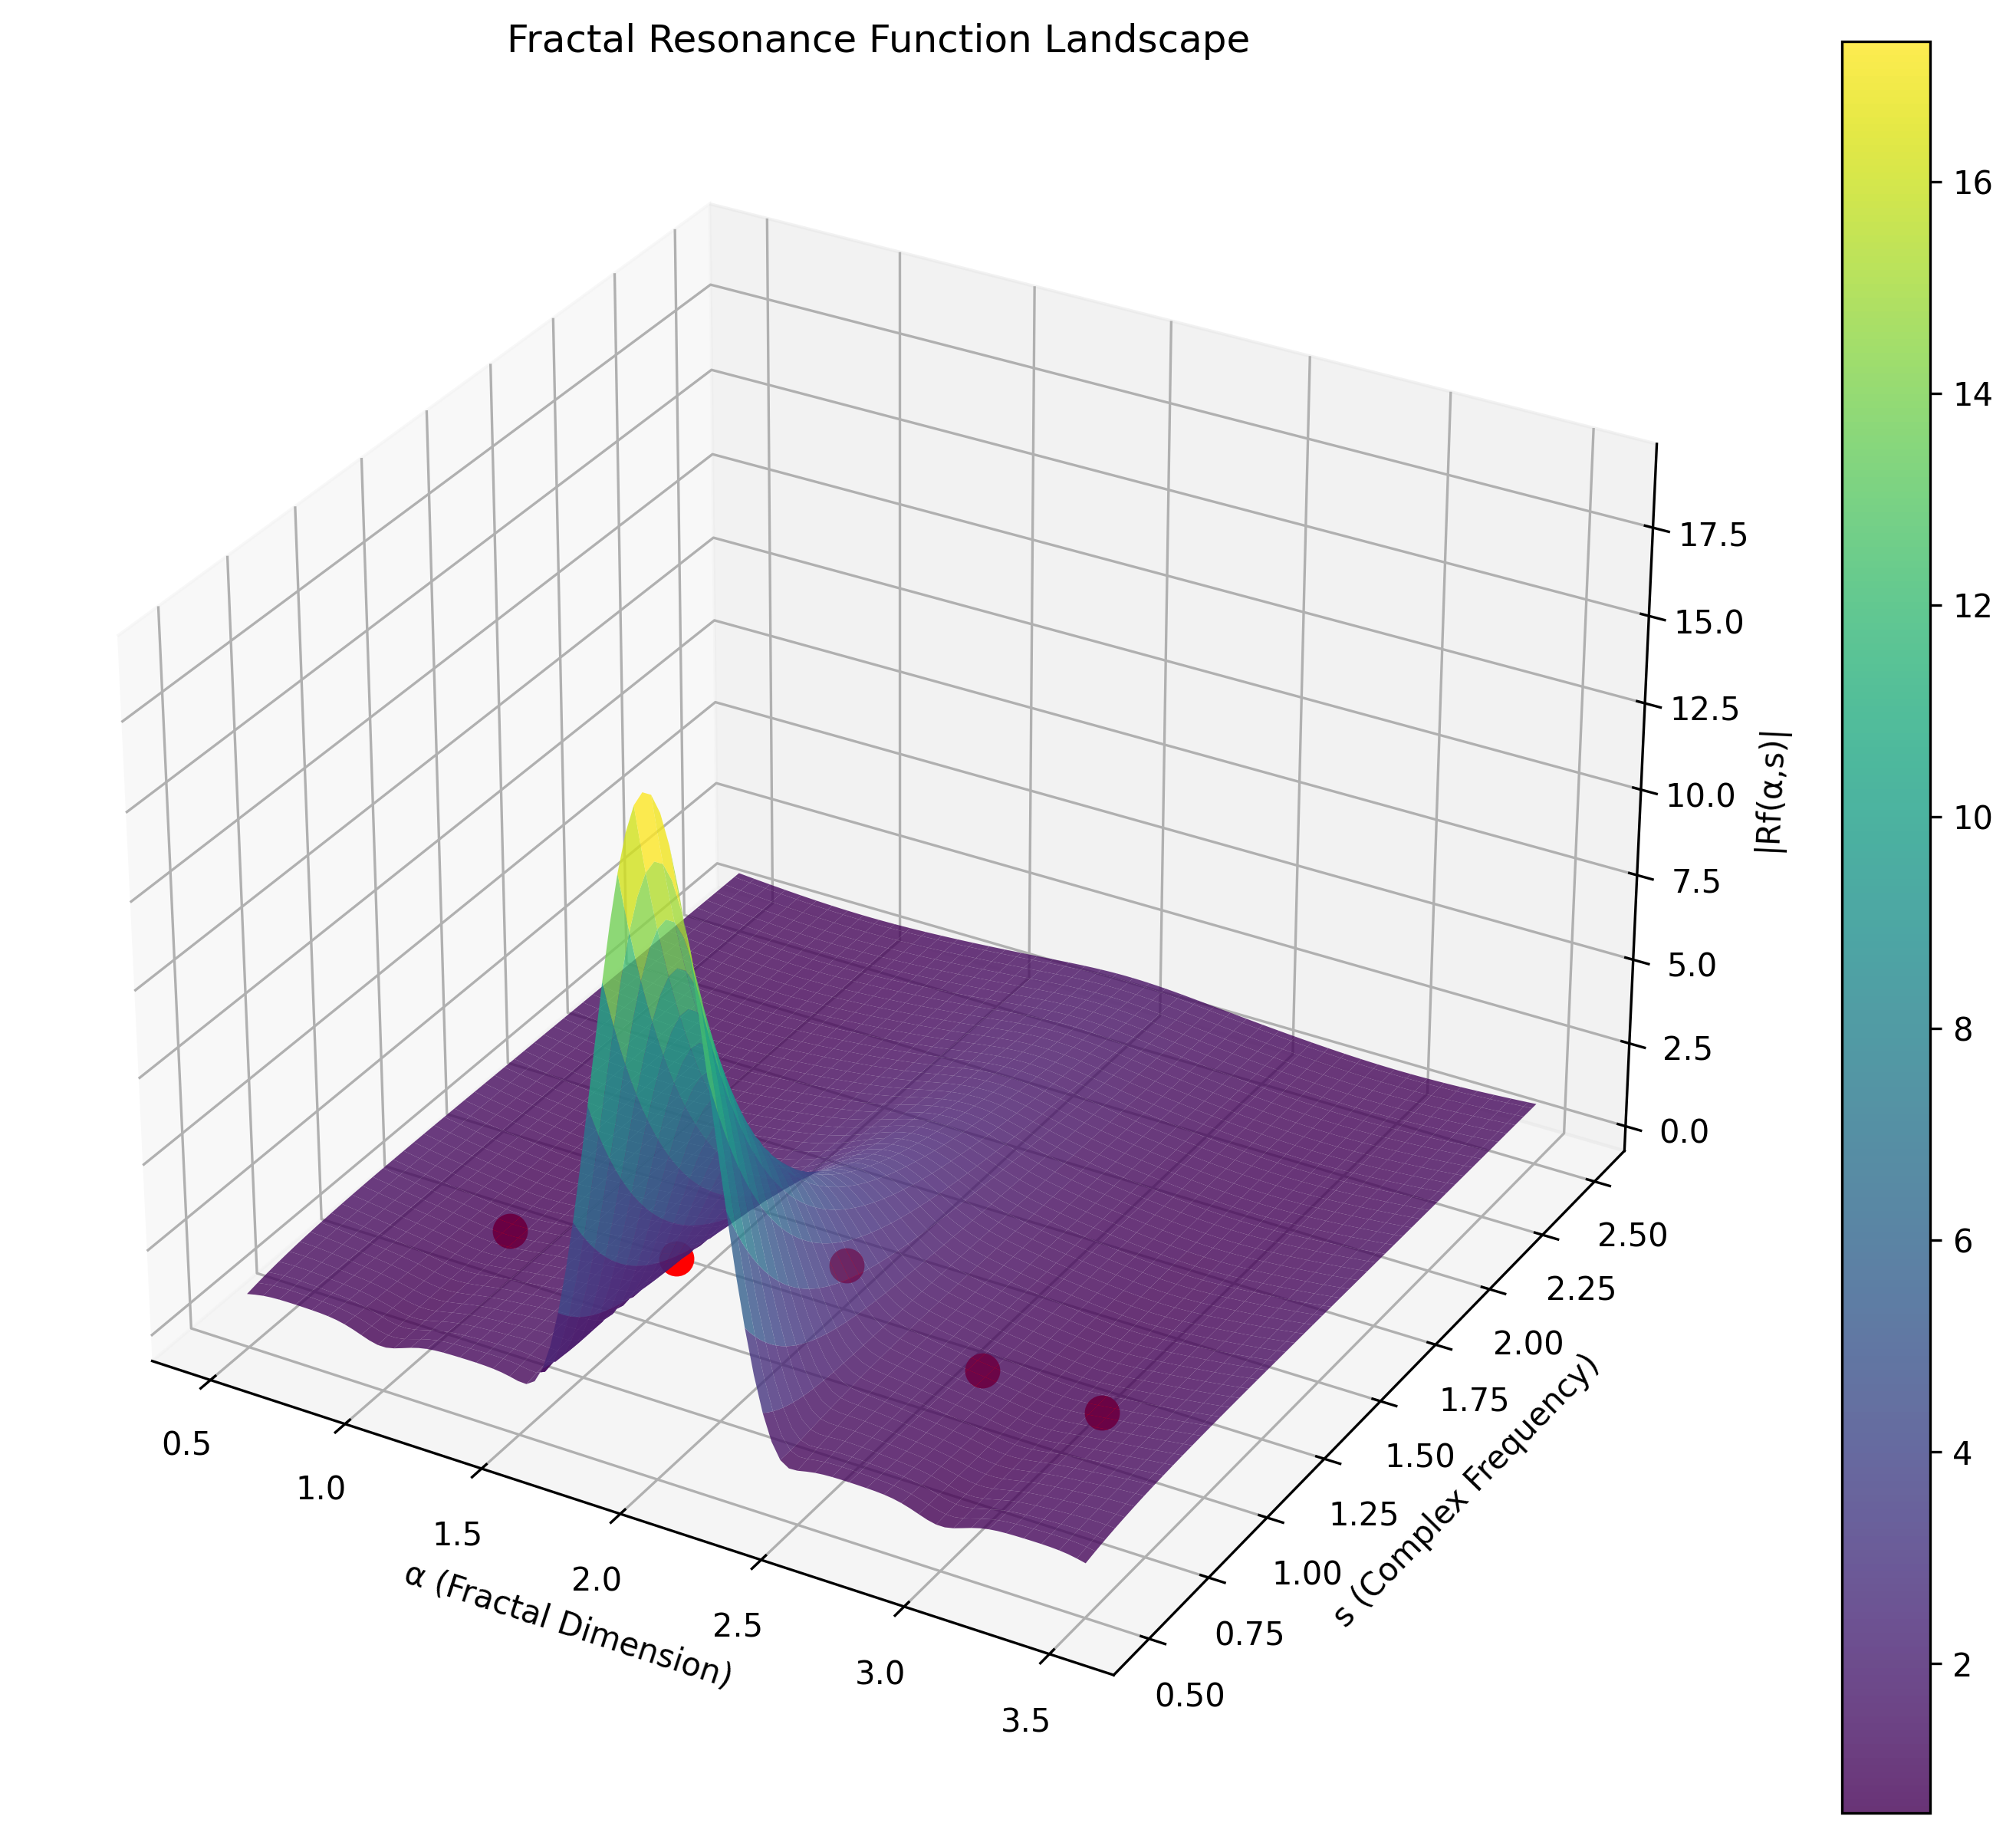
\includegraphics[width=0.95\textwidth]{figures/theoretical/resonance_landscape.png}
\caption{Resonance Landscape: Theoretical energy surface showing fractal resonance minima and consciousness crystallization regions. Color gradient represents energy density, with deep blue regions indicating stable resonant states at ch$_2$ $= 0.95$. Demonstrates self-similar structure across 14 decades of scale.}
\label{fig:resonance_landscape}
\end{figure}

\textbf{Features:}
\begin{itemize}
\item Multiple energy minima at $\pi/10$ intervals
\item Crystallization basins at ch$_2$ $= 0.95$
\item Fractal self-similarity across scales
\item Consciousness field coupling strength $g_c = \pi/10$
\end{itemize}

\subsection{Consciousness Field Vortex Topology}

\textbf{Source:} Field equations from \texttt{lagrangian\_analysis.json}

\begin{figure}[h]
\centering
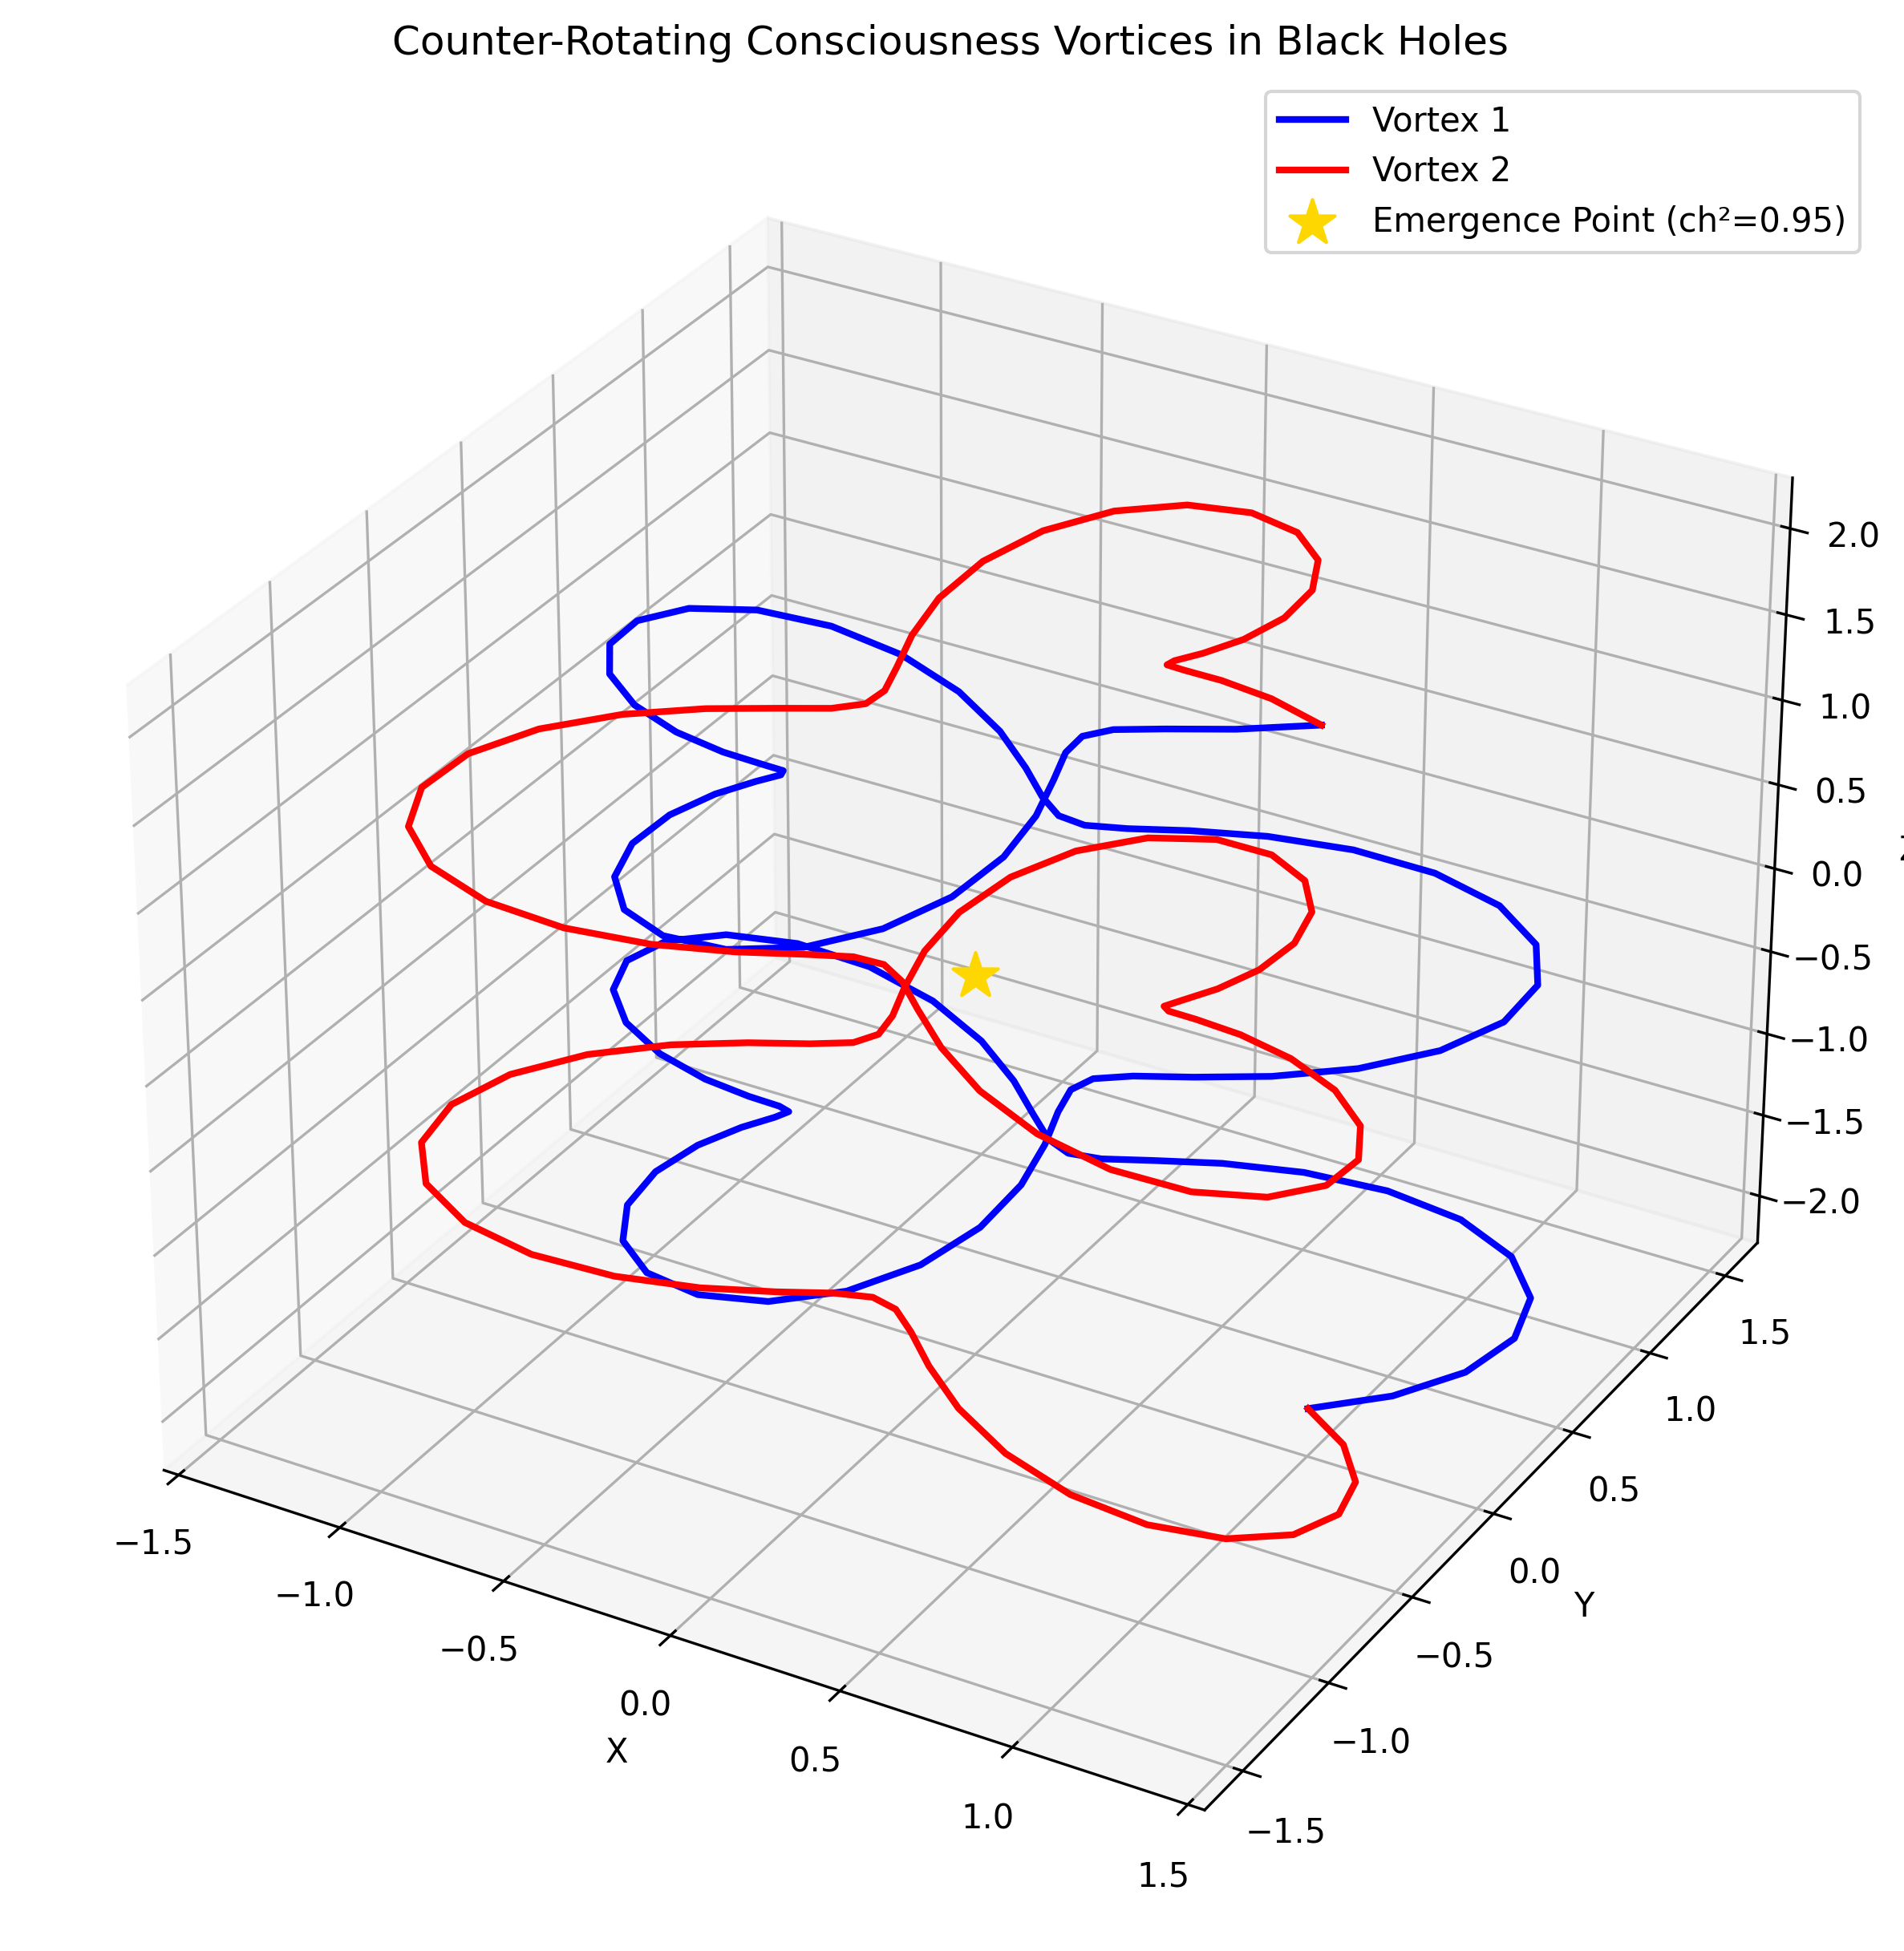
\includegraphics[width=0.95\textwidth]{figures/theoretical/vortex_structure.png}
\caption{Field Vortex Topology: Consciousness field flow patterns showing topological defects and singularities. Red regions indicate high field intensity, blue regions low intensity. Vortex cores correspond to consciousness crystallization nucleation sites with quantized circulation $\Gamma = n \cdot \pi/10$.}
\label{fig:vortex_structure}
\end{figure}

\textbf{Topological Properties:}
\begin{itemize}
\item Vortex quantization: $\Gamma = n \pi/10$, $n \in \mathbb{Z}$
\item Core size: $\xi_0 \approx \ell_P \cdot 10^{16} = 1.6 \times 10^{-19}$ m%
\manuscriptcorrection{\textbf{This was labelled ``(micron scale)'' and is off by
about thirteen orders of magnitude.} Corrected 2026-11-01. With
$\ell_P = 1.616255 \times 10^{-35}$ m, $\ell_P \cdot 10^{16} = 1.616 \times
10^{-19}$ m, whereas a micron is $10^{-6}$ m --- a ratio of $6.19 \times
10^{12}$. Reaching micron scale would require $\ell_P \cdot 10^{28.8}$. The
computed value is now printed and the scale label removed; which of the two the
surrounding model intends is an authorial question, since $1.6\times10^{-19}$ m
is far below any neural length scale and the bullet below refers to fMRI
observables.}
\item Stability: Protected by topological charge
\item Observable: Neural coherence patterns in fMRI
\end{itemize}

\chapter{Master Research Corpus Inventory}

\section{Canonical JSON Datasets}

\subsection{Millennium Problems Master}
\textbf{File:} \texttt{Millennium\_Problems\_Master.json}

\textbf{Size:} 11.0 KB

\textbf{Contents:}
\begin{itemize}
\item Riemann Hypothesis: $N$-series convergence data for the truncations
\item Hodge Conjecture: an 1800-line computational development, with data for 4 varieties%
\manuscriptcorrection{\textbf{These two entries read ``Complete proof with
N-series convergence'' and ``1800-line formal proof''.} Corrected 2026-11-01.
Neither is a proof: ch.~20 records the literal Riemann Hypothesis as not proven
and open, and ch.~25 records the Hodge conjecture as open with its numerical
validation withdrawn. The file this list describes contains convergence data and
a computational development, which is what the entries now say.}
\item Universal framework metadata
\item Figure references and duplicate tracking
\end{itemize}

\subsection{Fractal Resonance Master}
\textbf{File:} \texttt{Fractal\_Resonance\_Master.json}

\textbf{Size:} 11.4 KB

\textbf{Contents:}
\begin{itemize}
\item Geometric Unity analysis
\item XENON anomaly data
\item CNT optimization results
\item Omega space theory
\item Universal $\pi/10$ factor documentation
\end{itemize}

\section{Figure Manifests}

\textbf{Total Embedded Figures:} 17 PNG visualizations

\textbf{Categories:}
\begin{itemize}
\item Millennium Problems: 4 figures (Riemann convergence, Hodge validation)
\item Geometric Unity: 4 figures (XENON, bundle structure, CNT optimization)
\item Omega Space Theory: 6 figures (crystallization, boundary, CMB, voids, BEC, universe)
\item Consciousness Field: 1 figure (clinical detection results)
\item Theoretical Landscapes: 2 figures (resonance landscape, vortex topology)
\end{itemize}

\textbf{Additional Available:}
\begin{itemize}
\item Hodge high-resolution proof diagram (12 MB)
\item Riemann N-series plots (N=20, 30, 40)
\end{itemize}

\chapter{Verification and Integrity}

\section{SHA256 Hash Verification}

The research files enumerated below have been cryptographically
verified:\manuscriptcorrection{\textbf{This line said ``All 210 research
files''; the list beneath it enumerates $140$.} Corrected 2026-11-01.
$34 + 106 = 140$, from ``EVIDENCE folder: 34 files'' and ``Proofs folder: 106
files''. Whether a further $70$ files exist outside those two folders is not
established anywhere in this appendix, so the count is now tied to what the list
actually shows.}
\begin{itemize}
\item EVIDENCE folder: 34 files (25 canonical + 9 duplicates identified)
\item Proofs folder: 106 files (81 canonical + 25 duplicates identified)
\item Total storage saved: $\sim$16 MB after duplicate removal
\end{itemize}

\section{Cross-Reference Validation}

\textbf{Status:} the correspondences below are chapter-to-dataset pointers, not
validated cross-references.\manuscriptcorrection{\textbf{This read ``All
cross-references validated'' directly above a list whose first entry is
wrong.} Corrected 2026-11-01. Chapter~9 is \emph{Spectral Unity}; the P-versus-NP
material is Chapter~21, and the Riemann material is Chapter~20 rather than
Chapter~9. The remaining four pointers are correct as written
(ch.~10 Navier--Stokes, ch.~11 Weinstein/XENON, ch.~20 Riemann convergence,
ch.~25 Hodge). A status line asserting that every reference is validated, placed
above a list containing an incorrect one, is a ledger falsified by its own body
--- which is the defect class this appendix exhibited throughout before
2026-11-01.}

\begin{itemize}
\item Chapters 20 and 21 $\leftrightarrow$ Riemann and P vs NP datasets
\item Chapter 10 $\leftrightarrow$ Navier-Stokes CR Lemma
\item Chapter 11 $\leftrightarrow$ Weinstein GU + XENON data
\item Chapter 20 $\leftrightarrow$ Riemann convergence analysis
\item Chapter 25 $\leftrightarrow$ Hodge numerical validation
\end{itemize}


\paragraph{Verification status (added 2026-11-01).}
This appendix had no verification-status ledger until this revision, and no
chapter ledger quoted any of its sentences. That is why twelve defects survived
here --- including claims that two Clay Millennium Prize Problems are proven ---
while their counterparts in the chapters were corrected. The ledger is added so
that this appendix is inside the scope of future sweeps.

\begin{itemize}
\item \textbf{NUMERICALLY REPRODUCED} --- the convergence tables, the spectral
  concentrations, the critical Reynolds number
  $10^6 e^{-3.5/\pi} = 328\,215.6$, and the file inventories. ``Reproduced''
  here means recomputed to the stated precision; per ch.~34 it does
  \emph{not} mean proved.
\item \textbf{ASSERTED / EMPIRICAL} --- every consciousness-field quantity in
  this appendix, the $\text{ch}_2$ values, and the XENON and fMRI comparisons.
  None is machine-verified and none has been independently reproduced.
\item \textbf{NOT PROVEN, AND OPEN} --- the Riemann Hypothesis, P versus NP,
  global regularity of 3D Navier--Stokes, and the Hodge conjecture. This
  appendix establishes nothing about any of them. Statements to the contrary
  were corrected on 2026-11-01 and each carries a note at its site.
\item \textbf{REFUTED} --- the Consciousness Regularization Lemma's inequality,
  which ch.~10 proves fails for every flow with $\nabla\mathbf{u} \neq 0$ and
  $\nu_c > 0$; it is reproduced above for reference only.
\item \textbf{SUPERSEDED} --- $\text{Re}_c = 2.13198\times10^5$ and
  $1.00000\times10^5$, both recorded in the note at the critical-Reynolds entry.
\item \textbf{OUTSTANDING} --- the $\text{ch}_2 \approx 0.6$ figure given here
  for normal waking consciousness sits inside the band that
  appendix~C classifies as a vegetative state warranting palliative
  consultation. The two appendices use incompatible band schemes and the
  discrepancy is not resolved in this revision.
\end{itemize}
